\documentclass[conference]{IEEEtran}
\usepackage[T1]{fontenc}
\usepackage{cite}
\usepackage{amsmath,amssymb,amsfonts}
\usepackage{graphicx}
\usepackage{textcomp}
\usepackage{xcolor}
\usepackage{booktabs,tabularx,array}
\usepackage{url}
\usepackage[hidelinks]{hyperref}
\usepackage{microtype}
\usepackage{placeins}
\hypersetup{pdftitle={PLUME-Advanced: Methods and Measured Evaluation},
  pdfauthor={Anonymous Authors},pdfsubject={Measured Earth evaluation campaign with explicit limits}}

% Detailed illustrated draft. All active figure assets are bundled in figures/.
% Upload the entire ZIP and select main.tex with pdfLaTeX.
% Images are included directly: missing files produce an error, not an empty box.
\newcolumntype{Y}{>{\raggedright\arraybackslash}X}

\begin{document}

\title{PLUME-Advanced: Host-Conditioned Procedural Generation of Planetary Lava-Tube Environments for Robotics Simulation}
\author{Anonymous Authors}
\maketitle

\begin{abstract}
Robotic exploration of planetary lava tubes requires repeatable three-dimensional environments with controllable geometry, connectivity and hazards. We present PLUME-Advanced, a staged procedural framework that combines spatial host conditioning, directed networks, adaptive cross-sections, volumetric reconstruction, structural scenarios and portable scene packaging. An intrinsic floor atlas retains segment identity, vertical level and clearance after volume changes. The model is an inspectable procedural prior, not a thermofluid or geomechanical solver. A frozen-source Earth campaign attempted 2,076 cases across seven experiments; 2,071 completed and five dense 5 km reconstructions exceeded a 12 GiB memory budget. Against 200 reference contours from 19 evaluation caves, 100 generated worlds achieved a selected normalized morphometric distance of 0.254, versus 0.840 for dimension-matched ellipses, while size and variability mismatches remained. Tiled reconstruction completed all 20 resource cases. Routing interventions changed centerlines, but distributary tendency did not change median cycle rank. Adaptive sampling had higher point-set discrepancy in all 30 approximately count-matched comparisons. All 33 A--C repeatability checks passed and 15 target packages were emitted; application imports were not tested. These results delimit the current representation's behavior without establishing final-mesh fidelity, planetary interior distributions or robotics performance.
\end{abstract}

\begin{IEEEkeywords}
procedural generation, planetary robotics, lava tubes, subterranean environments, simulation, synthetic environments
\end{IEEEkeywords}

\section{Introduction}
Planetary lava tubes are of interest as geological archives, exploration targets, and potential sheltered environments. Comparative analysis of terrestrial surveys and planetary surface features suggests that some lunar and Martian cavities may be substantially larger than familiar terrestrial passages \cite{sauro2020}. Radar observations at the Mare Tranquillitatis pit provide evidence for a subsurface conduit connected to a lunar pit \cite{carrer2024}. Such observations strengthen the motivation for subsurface exploration, but they do not provide the dense interior geometry, traversability maps, or distributions of passage shapes needed to design and evaluate autonomous robots.

An exploration robot must operate with limited illumination, unavailable satellite navigation, restricted viewpoints, and uncertain local terrain. Junctions create route ambiguity; geometrically similar corridors challenge place recognition; debris and constrictions affect clearance; and vertically overlapping passages complicate maps based on horizontal projection. Communication and recovery can become more difficult as the robot moves away from an entrance. These conditions motivate controlled simulation experiments in which the environment can be varied independently of the autonomy algorithm \cite{cano_navigation,daedalus2021}.

A small set of manually authored meshes cannot expose the full range of these conditions. Conversely, generating many visually varied caves is insufficient if their topology is difficult to interpret, hazards do not affect collision geometry, or changes in one parameter unpredictably alter the entire scene. Scientific use therefore requires both diversity and experimental control. A useful generator should retain information about where passages connect, which conditions influenced their placement, how geometry was reconstructed, and whether the final accessible space still agrees with the original network.

PLUME \cite{plume2025} established a graph-based procedural workflow for underground environments intended for robotics simulation. PLUME-Advanced develops that approach around an explicit spatial host representation and retained semantic artifacts. Its purpose is not to reconstruct a particular surveyed cave or predict the outcome of a volcanic eruption. Instead, it creates an ensemble of conditional environments that can be inspected, modified, and reused as experimental stimuli.

The research question is whether this combination can support a controllable environment prior spanning network structure, cross-sectional morphology, structural scenarios, and simulator packaging. The design is motivated by three requirements. First, geological inputs should have identifiable consumers in generation rather than serve only as labels. Second, topology and geometry should remain coupled but separately inspectable. Third, changes introduced after network construction must be reflected in the geometry and metadata supplied to robotics applications.

The contributions of this work are:
\begin{enumerate}
\item An explicit host-conditioning interface with decomposable routing penalties, reproducible parameter interventions, and separate formation and structural-survival controls.
\item An integrated network-to-volume representation combining multi-source directed flow semantics, persistent split and merge structure, adaptive three-dimensional sections, and local structural modifications.
\item A topology-aware floor atlas and canonical scene workflow that retain semantic identity, distinguish formation connectivity from final free space, and support reproducible evaluation and multiple export packages.
\end{enumerate}
These contributions concern the integration and inspectability of a lava-tube scenario generator. Geological conditioning of cave networks, graph skeletons, and implicit geometry individually have substantial prior art. Claims of improved morphology, efficiency, or portability require the measurements specified in Section~\ref{sec:experiments}.

\section{Related Work}
\subsection{Planetary Observations and Structural Models}
Terrestrial caves provide direct measurements of lava-tube interiors, whereas planetary interpretation relies heavily on surface morphology and remote sensing. Sauro \emph{et al.}\ \cite{sauro2020} compare terrestrial, lunar, and Martian tube-related features and discuss their scale differences. Carrer \emph{et al.}\ \cite{carrer2024} constrain a conduit beneath a lunar pit using radar observations. The evidence motivates scenario generation across different scales, while leaving major uncertainty in the interior geometry and network organization of individual planetary systems.

Structural feasibility is a separate question from formation size. Blair \emph{et al.}\ \cite{blair2017} use finite-element models to show sensitivity to roof thickness and assumed stress state. Chwa\l{}a \emph{et al.}\ \cite{chwala2024} examine variable cross-sectional geometry and its implications for failure. These studies do not justify scaling all cave dimensions with one gravity factor. PLUME-Advanced consequently treats body presets as configurable scenario envelopes and uses a local screening surrogate to expose structural sensitivity. Passing that screen does not establish engineering safety or validate the formation model.

\subsection{Procedural Cave and Underground Generation}
Cellular automata can produce cave-like level layouts at low computational cost \cite{johnson2010}. Volumetric terrain methods support cavities that cannot be represented by a single height surface \cite{santamaria2014}, while schematic maps and L-systems offer control over underground layout \cite{antoniuk2016}. These approaches motivate different representations for discrete connectivity and continuous geometry.

Geological conditioning is already central to the karst-network method of Paris \emph{et al.}\ \cite{paris2021}. Their skeleton construction incorporates geological constraints and is converted into implicit conduit geometry. This is an important precedent for spatially conditioned network generation. The present work addresses a different setting: lava-tube scenarios with procedural supply history, body-dependent operating envelopes, local roof screening, and retained information for robotics. It does not claim that host-conditioned cave synthesis itself is new.

For robotics, Cano \emph{et al.}\ \cite{cano_gazebo} assemble randomized underground environments for Gazebo using reusable modules. Their navigation work illustrates the utility of topological instructions and corridor/intersection recognition \cite{cano_navigation}. PLUME \cite{plume2025} instead offers a graph-driven workflow for creating underground meshes. These systems establish the value of varied synthetic environments, while motivating finer control over continuous morphology and the relationship between spatial host fields and network structure.

\subsection{Empirical and Parametric Lava-Tube Modelling}
Pyroduct \cite{pyroduct2026} is a parametric lava-tube generator developed for Grasshopper in Rhinoceros. It draws on terrestrial cross-sectional morphology and supports terrestrial and planetary modelling. The associated Pyroduct Digital Catalog (PDC) provides digitized terrestrial sections and source metadata \cite{pdc2025}. Together, the software and catalog provide relevant prior work and an external geometric reference.

PLUME-Advanced emphasizes stochastic network-scale scenarios and retained simulation semantics. This focus is complementary to empirical parametric modelling; it does not establish superiority over Pyroduct. A comparison against a simple ellipse tests the value of a profile family, not performance against the complete Pyroduct system. A future direct software comparison would require matched inputs, compatible outputs, and an agreed definition of the task.

\begin{table*}[t]
\caption{Positioning by documented emphasis. This is a scope comparison, not a benchmark or a claim that an unlisted capability is absent.}
\label{tab:related}
\centering\small
\begin{tabularx}{\textwidth}{@{}p{2.65cm}YYY@{}}
\toprule
Approach & Principal representation & Documented emphasis & Relation to this work \\
\midrule
Cellular automata \cite{johnson2010} & Discrete cave-like level layout & Fast procedural level generation & Motivates inexpensive diversity \\
Paris \emph{et al.}\ \cite{paris2021} & Conditioned skeleton and implicit conduits & Geological coherence of karst networks & Precedent for geological network conditioning \\
Cano \emph{et al.}\ \cite{cano_gazebo} & Assembly of underground modules & Randomized Gazebo environments & Simulator-oriented environment generation \\
PLUME \cite{plume2025} & Graph and generated underground mesh & Flexible environments for space robotics & Predecessor workflow \\
Pyroduct \cite{pyroduct2026} & Parametric lava-tube geometry & Empirical cross-sectional morphology & Domain-specific reference and comparison context \\
PLUME-Advanced & Host fields, graph, sections, volume, atlas & Inspectable networked scenarios and portable assets & Integrated system evaluated in this paper \\
\bottomrule
\end{tabularx}
\end{table*}

\section{Problem Formulation and Design Requirements}
\label{sec:formulation}
Let $\boldsymbol{\theta}$ denote a resolved configuration containing the body and material preset, host parameters, network controls, section-shape parameters, volumetric resolution, event settings, and export choices. A master seed $z$ determines stochastic variation. The generator produces
\begin{equation}
\mathcal{A}=F(\boldsymbol{\theta},z),\qquad
\mathcal{A}=\{\mathcal{M}_v,\mathcal{M}_c,\mathcal{G},\mathcal{I},\mathcal{P}\},
\label{eq:asset}
\end{equation}
where $\mathcal{M}_v$ is visual geometry, $\mathcal{M}_c$ is collision geometry, $\mathcal{G}$ is the formation graph, $\mathcal{I}$ is the intrinsic floor atlas, and $\mathcal{P}$ contains configuration, provenance, and semantic metadata. This notation describes the logical canonical asset; individual exporters may place these components in separate files.

The output must satisfy several distinct requirements. \emph{Repeatability} concerns whether the same inputs reproduce the same semantic environment in a recorded software environment. \emph{Controllability} concerns whether a declared intervention changes an interpretable property. \emph{Representation fidelity} concerns whether the volume and mesh preserve the intended passages at a chosen resolution. \emph{Portability} concerns whether an exported package preserves canonical scale and asset identity after import. None of these alone establishes geological validity.

We use ``causal'' only in the operational sense of the software dependency graph. Holding a seed fixed while changing a routing weight identifies an intervention within this generator. It does not identify a causal law of volcanic emplacement. Likewise, conservation of a procedural flux label is an internal consistency property; it does not imply conservation of energy, solution of momentum balance, or prediction of an eruption history.

Three connectivity concepts are distinguished throughout. The directed formation graph records how generated conduits are related. The reconstructed free-space topology follows from the density field after structural modifications. Robot traversability additionally depends on body dimensions, kinematics, slope, contact, and sensing. A graph edge can remain in the formation record even when a collapse blocks its volume, and a connected void can still be impassable to a particular robot.

\section{PLUME-Advanced}
\label{sec:method}
\subsection{Staged Architecture and Reproducibility}
The canonical frame is right-handed, Z-up, and metric. Host generation, network construction, section sampling, events, and appearance use named random domains derived from the master seed. The implementation combines a stable encoding of the domain labels with NumPy seed-sequence generation, avoiding dependence on the process-randomized Python hash. Labels can include a stage and a persistent semantic identifier, allowing local variation without consuming one global sequence of random draws.

The logical data flow is
\begin{equation}
\begin{split}
\mathcal{H}&\longrightarrow\mathcal{G}\longrightarrow\mathcal{S}
\longrightarrow\mathcal{V}_0\longrightarrow\mathcal{V}_*,\\
\mathcal{V}_*&\longrightarrow(\mathcal{M},\mathcal{I}_*)
\longrightarrow\mathcal{A},
\end{split}
\label{eq:pipeline}
\end{equation}
where $\mathcal{H}$ is the host, $\mathcal{S}$ the section field, $\mathcal{V}_0$ the constructed base volume, and $\mathcal{V}_*$ the volume after structural processing. Figure~\ref{fig:pipeline} distinguishes the conceptual stages from their execution order. Geometry is first available as a queryable density field; optional events use that field; the final wall is then meshed. A final atlas is refreshed against the modified volume.

This organization matters for reproducibility. Changing an event seed should preserve the host, network, and sections, but may alter the final volume and atlas. Changing an export target should preserve the canonical asset. Stage-specific seeds make such isolation possible, but do not by themselves prove it: semantic hashes and explicit intervention tests are required. Reproduction across dependency versions or numerical platforms is recorded separately from reproduction in one fixed environment.

\begin{figure*}[t]
\centering
\includegraphics[width=\textwidth,height=49mm,keepaspectratio]{figures/f01_pipeline.pdf}
\caption{PLUME-Advanced data flow. Stage D is executed in construction and meshing passes so that structural changes affect the final cave boundary. The formation graph and stage artifacts remain inspectable; the floor atlas is refreshed after volume modification. The diagram describes software dependencies, not a physically simulated sequence of volcanic processes.}
\label{fig:pipeline}
\end{figure*}

\subsection{Spatial Host Representation}
Stage A constructs a low-frequency host slab over a horizontal domain $\Omega_H\subset\mathbb{R}^2$. Its fields include terrain elevation $h$, slope, emplacement thickness, cover $H_c$, lithological quality, fracture intensity $F_r$, flow capacity $K_f$, deposits, erosion, roof competence $Q_r$, and roof stability $S_r$. A source region, dominant flow direction, broad grade, spatial correlation scales, and coherent perturbations produce a spatially structured substrate. This representation is a two-dimensional field stack queried by subsequent three-dimensional construction; it is not a full three-dimensional stratigraphic or volcanic-edifice model.

Field roles are intentionally separated. Emplacement thickness and the host corridor influence carrying capacity. Fracture and erosion reduce competence. Cover influences both routing preference and structural demand. Bilinear queries provide continuous values between grid samples. The field names convey the intended procedural interpretation, while the resolved configuration defines their actual numerical construction.

The host-scale demand proxy is
\begin{equation}
D_H(x,y)=\frac{\rho g W_c^2}
{\max(H_c(x,y),\epsilon_H)\,\sigma_{\mathrm{eff}}},
\label{eq:demand}
\end{equation}
where $\rho$ is rock density, $g$ gravitational acceleration, $W_c$ a characteristic span, and $\sigma_{\mathrm{eff}}$ effective tensile strength. Here $\epsilon_H$ has units of length; the implementation uses a small positive cover floor. The ratio is dimensionless because $\rho gW_c^2/H_c$ has units of stress. The corresponding stability prior is
\begin{equation}
S_r(x,y)=\operatorname{clip}\!\left(
\frac{Q_r(x,y)}{1+D_H(x,y)},0,1\right).
\label{eq:stability}
\end{equation}
This field influences route preference before actual sections exist. It is distinct from the later geometry-specific roof screen in Section~\ref{sec:roof}.

\begin{table}[t]
\caption{Default routing penalties. Weights are procedural defaults, not fitted geological constants.}
\label{tab:host}
\centering\small
\begin{tabularx}{\columnwidth}{@{}lYr@{}}
\toprule
Term & Penalty increasing with & Weight \\
\midrule
$C_s$ & Normalized terrain slope & 0.12 \\
$C_c$ & Insufficient cover & 0.10 \\
$C_f$ & Fracture intensity & 0.22 \\
$C_q$ & Low flow capacity & 0.28 \\
$C_r$ & Low roof stability & 0.28 \\
\bottomrule
\end{tabularx}
\end{table}

Network steering consumes
\begin{equation}
C(x,y)=\sum_{j\in\{s,c,f,q,r\}}\bar{w}_j C_j(x,y),
\quad \bar{w}_j=\frac{w_j}{\sum_k w_k},
\label{eq:routing}
\end{equation}
under the default normalized-weight configuration. The terms lie in $[0,1]$; capacity and stability penalties are $1-K_f$ and $1-S_r$. Cover is normalized relative to minimum stable cover and layer thickness, while slope uses a percentile-based normalization. The five default weights in Table~\ref{tab:host} sum to one. Disabling routing conditioning replaces this scalar by a spatial constant. Setting one weight to zero renormalizes the remaining terms when normalization is enabled.

Figure~\ref{fig:host} illustrates selected host fields. The model records individual weighted contributions, enabling inspection of whether a term varies spatially and whether routes respond to it. A weak effect can arise because a term is nearly constant, correlated with another field, or dominated by other routing mechanisms. In particular, removing the explicit fracture penalty does not remove fracture influence already propagated into competence and capacity. The corresponding experiment is therefore a \emph{routing-term ablation}, not a complete removal of fracture information.

\begin{figure*}[t]
\centering
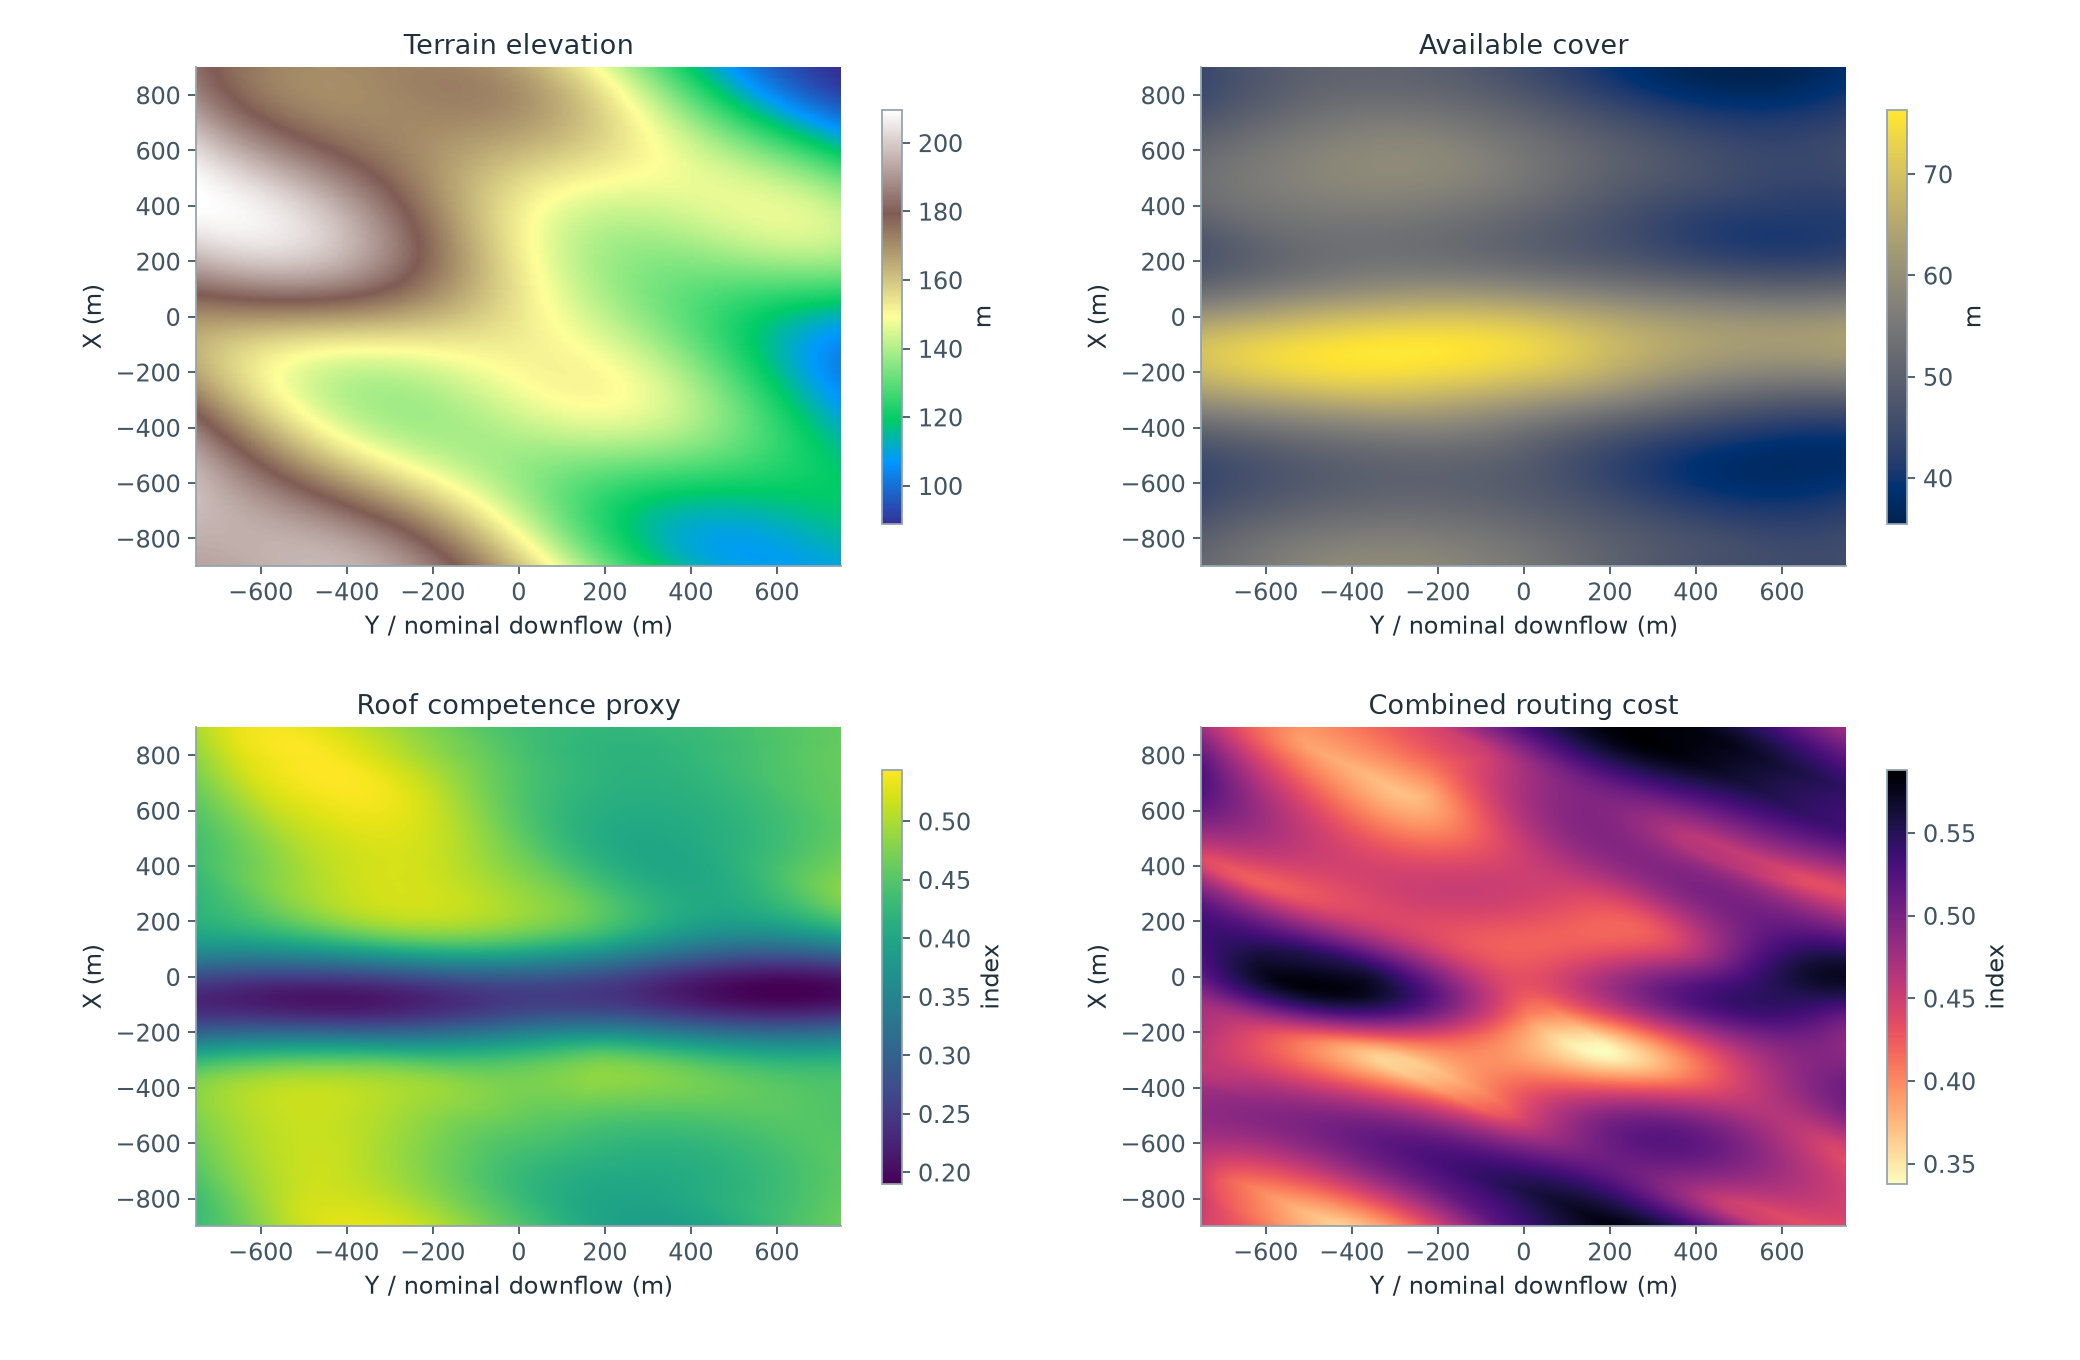
\includegraphics[width=\textwidth,height=112mm,keepaspectratio]{figures/f02_host_fields.png}
\caption{Illustrative host fields for the saved Earth inspection scenario, seed 4: terrain elevation, available cover, roof competence, and combined routing cost. The host was reconstructed from the saved configuration for the documentation figure. Coordinates and dimensional fields are in metres; competence and routing cost are indices. This single realization illustrates the inputs to routing, without establishing a matched-ablation effect.}
\label{fig:host}
\end{figure*}

\subsection{Network Growth and Procedural Emplacement History}
Stage B produces a directed graph $\mathcal{G}=(V,E)$ with entry, exit, junction, and terminal semantics. Edges retain ordered centerline points, segment identity, role, width estimates, host samples, and vertical-level labels. The current generator constructs multiple source feeders and one designated exit, while retaining retired or blind branches. Explicit connectivity supports inspection independently of the final mesh.

The current network model is richer than a fixed arrangement of decorative side branches. A terrain-guided backbone is combined with seeded lobe fronts and process-labelled emplacement phases. Candidate fronts diverge, compete for a finite phase supply, cool, retire, or coalesce into established downstream channels. Later phases may reoccupy an existing route. Metadata retain birth and death phases, allocated supply, formation state, and reoccupation or coalescence relationships. These labels provide a procedural history with tunable persistence; they do not resolve free-surface lava dynamics or physically timed eruption phases.

Several mechanisms affect the resulting structure. Distributary tendency changes opportunities for lateral growth. Duration and supply influence the resolved scenario extent and persistence. Inflation controls local enlargement, while host routing affects which alternatives are favored. Drained-pool chamber annotations represent selected widened regions associated with changes in local transport conditions. These parameters can interact, so a body-preset comparison cannot be interpreted as a gravity-only intervention.

A split followed by a downstream merge creates an alternative route in the underlying undirected graph without requiring a directed cycle. Directed acyclicity permits ordered state propagation; the undirected cycle rank measures route redundancy. Figure~\ref{fig:network} illustrates a saved formation network and its longitudinal floor/roof data. The implementation validates graph references and flow structure before section construction. Whether a geometrically reconstructed braid remains distinct must be checked later, since broad sections or insufficient separation can accidentally unite neighboring passages.

\begin{figure*}[t]
\centering
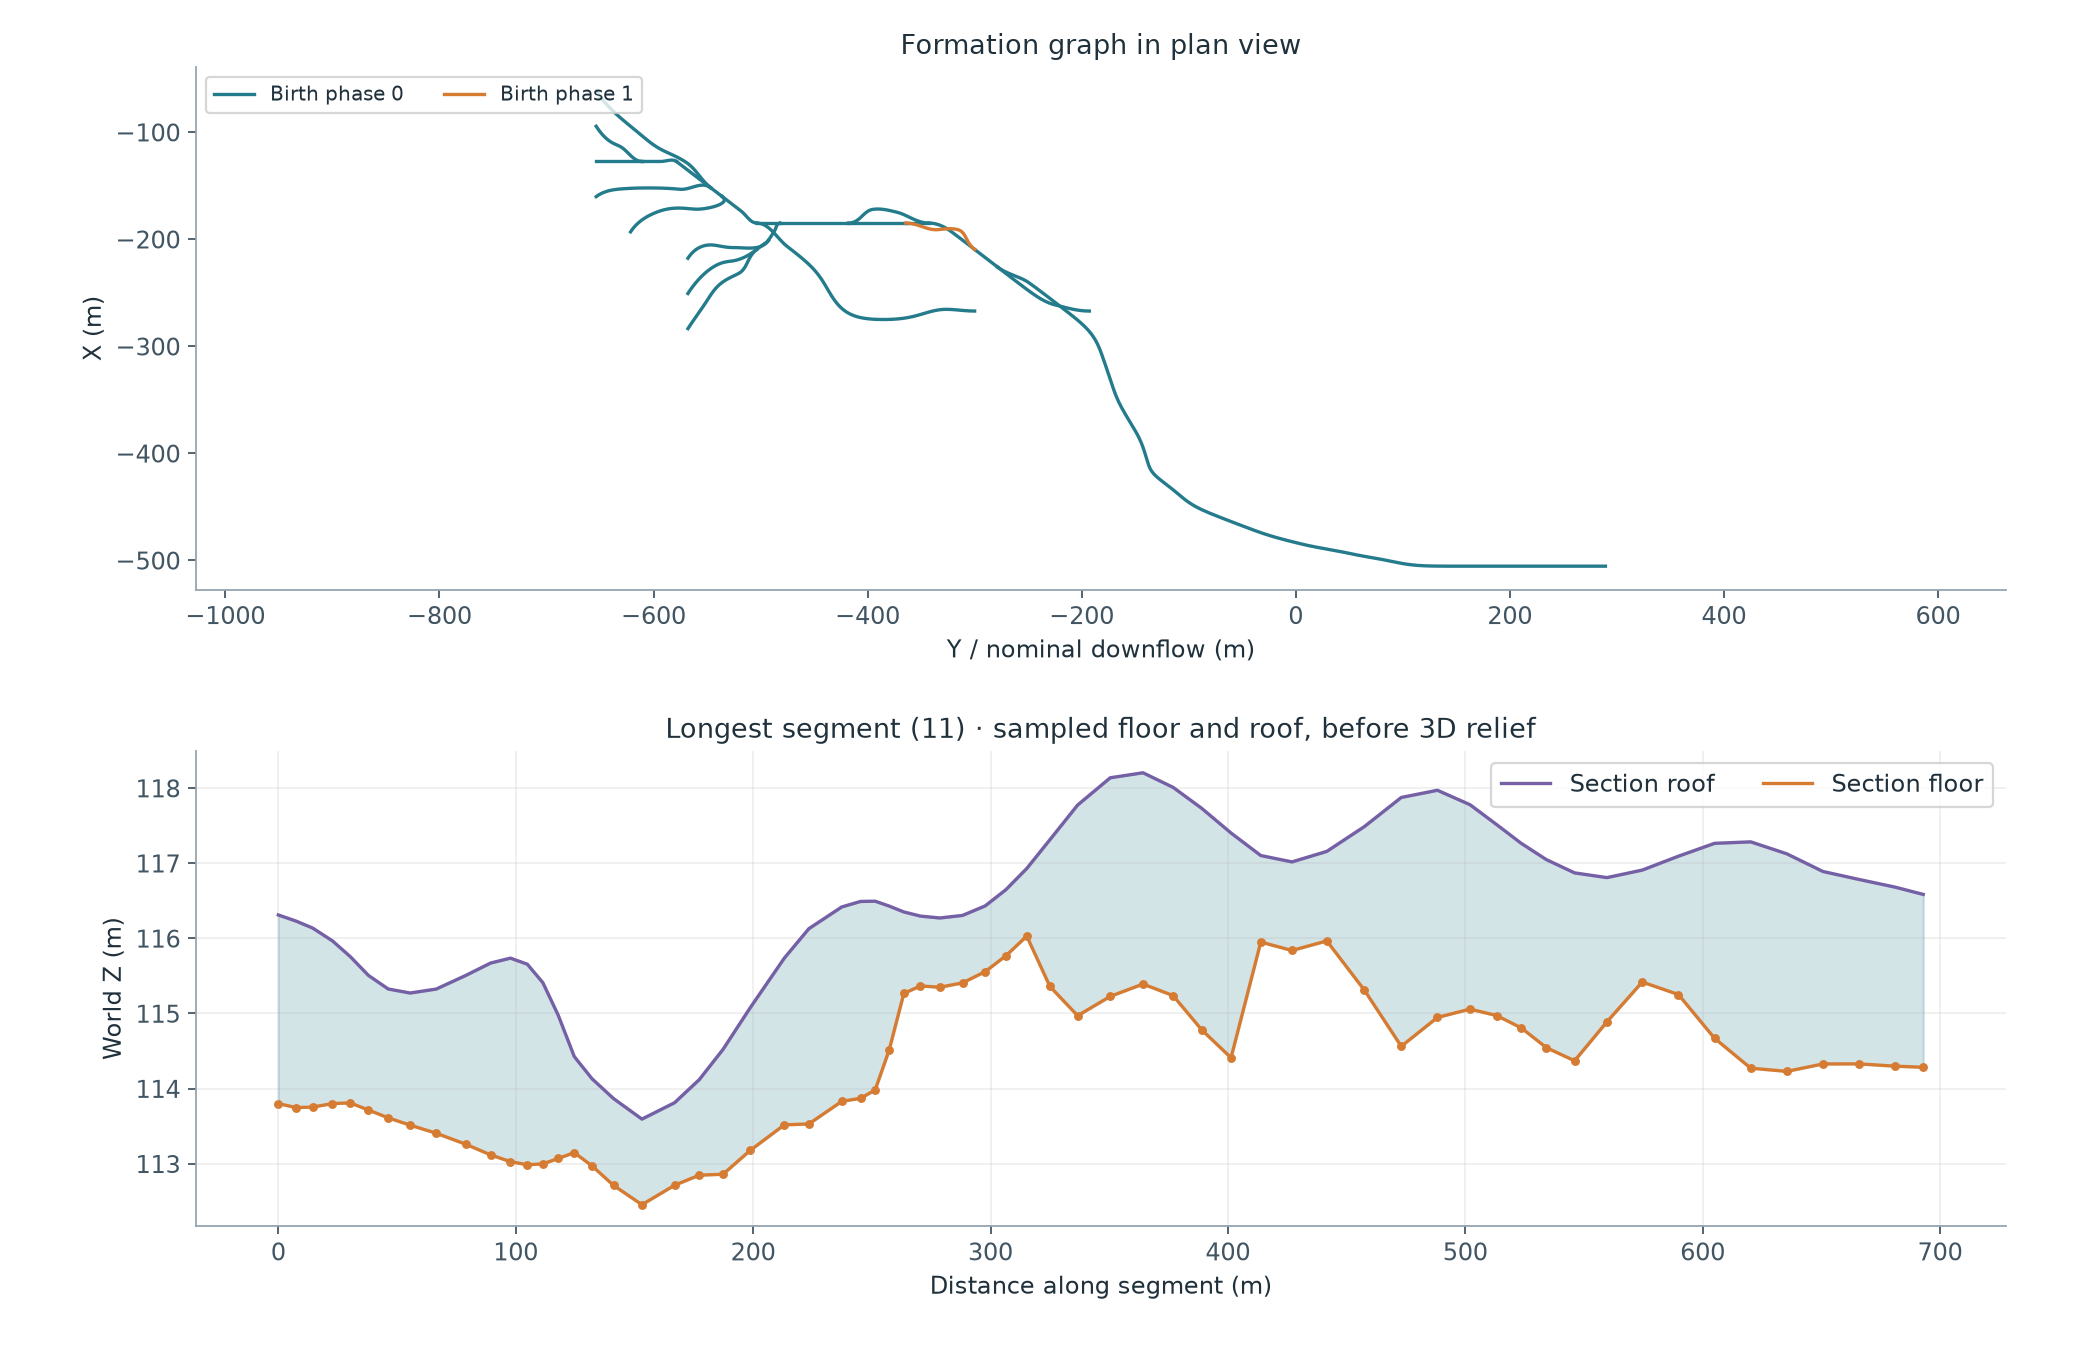
\includegraphics[width=\textwidth,height=112mm,keepaspectratio]{figures/f03_network.png}
\caption{Formation network and longitudinal section data for the saved Earth inspection scenario, seed 4. The plan view colors segments by birth phase. The lower panel follows the longest segment (ID 11) and shows sampled floor and roof elevations before three-dimensional surface relief. Vertical changes in that panel are exaggerated for readability; the plan view uses equal metric axes.}
\label{fig:network}
\end{figure*}

\subsection{Conserved Flux and Flow-State Propagation}
Each segment carries a procedural flux $q_e$, temperature $T_e$, and age $\tau_e$. Sources have independently seeded strengths influenced by inlet capacity; their total supply is normalized by the configured source-flux convention. Internal junctions obey
\begin{equation}
\sum_{e\in E^-(v)}q_e=\sum_{e\in E^+(v)}q_e.
\label{eq:flux}
\end{equation}
Equation~\eqref{eq:flux} applies to internal flow junctions. Sources inject supply, while exits and retired terminal structures are sinks in the procedural bookkeeping. Applying the equality without source or sink terms at every vertex would be incorrect.

Outgoing allocations are proportional to squared mean passage width at the allocation step:
\begin{equation}
q_e=Q_v\frac{\widehat{W}_e^{\,2}}
{\sum_{j\in E^+(v)}\widehat{W}_j^{\,2}},
\label{eq:allocation}
\end{equation}
where $Q_v$ is available supply and $\widehat{W}$ is the pre-adjustment mean width with a positive lower bound. Subsequent width adjustment is bounded. This is a carrying-capacity heuristic, not a discharge law derived from viscosity, hydraulic radius, or pressure gradients.

At a merge, incoming endpoint states are flux-weighted:
\begin{equation}
T_v=\frac{\sum_{e\in E^-(v)}q_eT_e^{\mathrm{end}}}{Q_v},
\quad
\tau_v=\frac{\sum_{e\in E^-(v)}q_e\tau_e^{\mathrm{end}}}{Q_v}.
\label{eq:mixing}
\end{equation}
Along a segment at distance $s$, the current propagation is
\begin{equation}
T_e(s)=\max(T_{\min},T_v-k_Ts),\qquad
\tau_e(s)=\tau_v+s/v_0,
\label{eq:cooling}
\end{equation}
with configured cooling rate $k_T$ and nominal speed $v_0$. Temperature decreases and age increases \emph{within} each segment. Mixing at a merge may raise temperature relative to a colder inlet or reduce age relative to an older inlet; global monotonicity relative to every incoming path is not claimed. Derived maturity and flow labels subsequently influence section morphology and event ranking. They are retained for interpretation rather than presented as measured thermal states.

\subsection{Three-Dimensional Placement and Adaptive Sections}
Stage C converts each ordered centerline into underground samples. A sample stores its center $\mathbf{c}_e(s)$, tangent $\mathbf{t}$, lateral axis $\mathbf{n}$, upward section axis $\mathbf{b}$, profile coordinates, dimensions, floor and roof information, and inherited flow state. A local profile point $(u,v)$ maps to world coordinates as
\begin{equation}
\mathbf{x}_e(s,u,v)=\mathbf{c}_e(s)+u\mathbf{n}_e(s)+v\mathbf{b}_e(s).
\label{eq:frame}
\end{equation}
For nonvertical tangents, the upward axis follows the projection of world Z into the normal plane. A fallback handles nearly vertical tangents. Keeping the roof-oriented axis upward prevents an apparent frame-continuity correction from exchanging the roof and floor. It also preserves the meaning of asymmetric roof profiles and floor incision during bends and elevation changes.

Figure~\ref{fig:geometry} shows selected profile envelopes. The section family independently controls width, height, roof arch, floor flatness, asymmetry, wall and floor relief, benches, and incised floor regions. Bounded segment-scale variation and smooth longitudinal modulation avoid assigning an independent unrelated shape at each sample. Profile construction retains the distinction between roof geometry and floor features: a lowered floor channel need not imply an equally displaced roof. Junction-aware blending tapers local parameters and adds support around connected segments.

Sampling density responds to the underlying centerline and profile variation:
\begin{equation}
\Delta s=\operatorname{clip}\!\left(
\frac{\Delta s_{\max}}{1+w_\kappa\kappa+w_wG_w+w_jJ},
\Delta s_{\min},\Delta s_{\max}\right).
\label{eq:adaptive}
\end{equation}
Here $\kappa$ is the implemented local turning measure, $G_w$ a width-gradient estimate, and $J$ a junction-proximity factor. The weights absorb the units of their estimators so that the denominator is dimensionless. The notation does not imply an exact differential-curvature formula. Segment endpoints are retained, and the spacing bounds prevent excessive or insufficient sampling. Uniform and dense reference policies provide alternative samples of the same procedural profile construction for evaluation.

Vertical-level labels are resolved into physical separation using actual passage dimensions and a rock-clearance allowance. A plan-view crossing is not automatically a junction. Nevertheless, the level label is metadata, not a geometric guarantee: final density connectivity must be inspected around crossings, especially where width or height increases or where junction blending extends beyond the nominal profile.

\begin{figure*}[t]
\centering
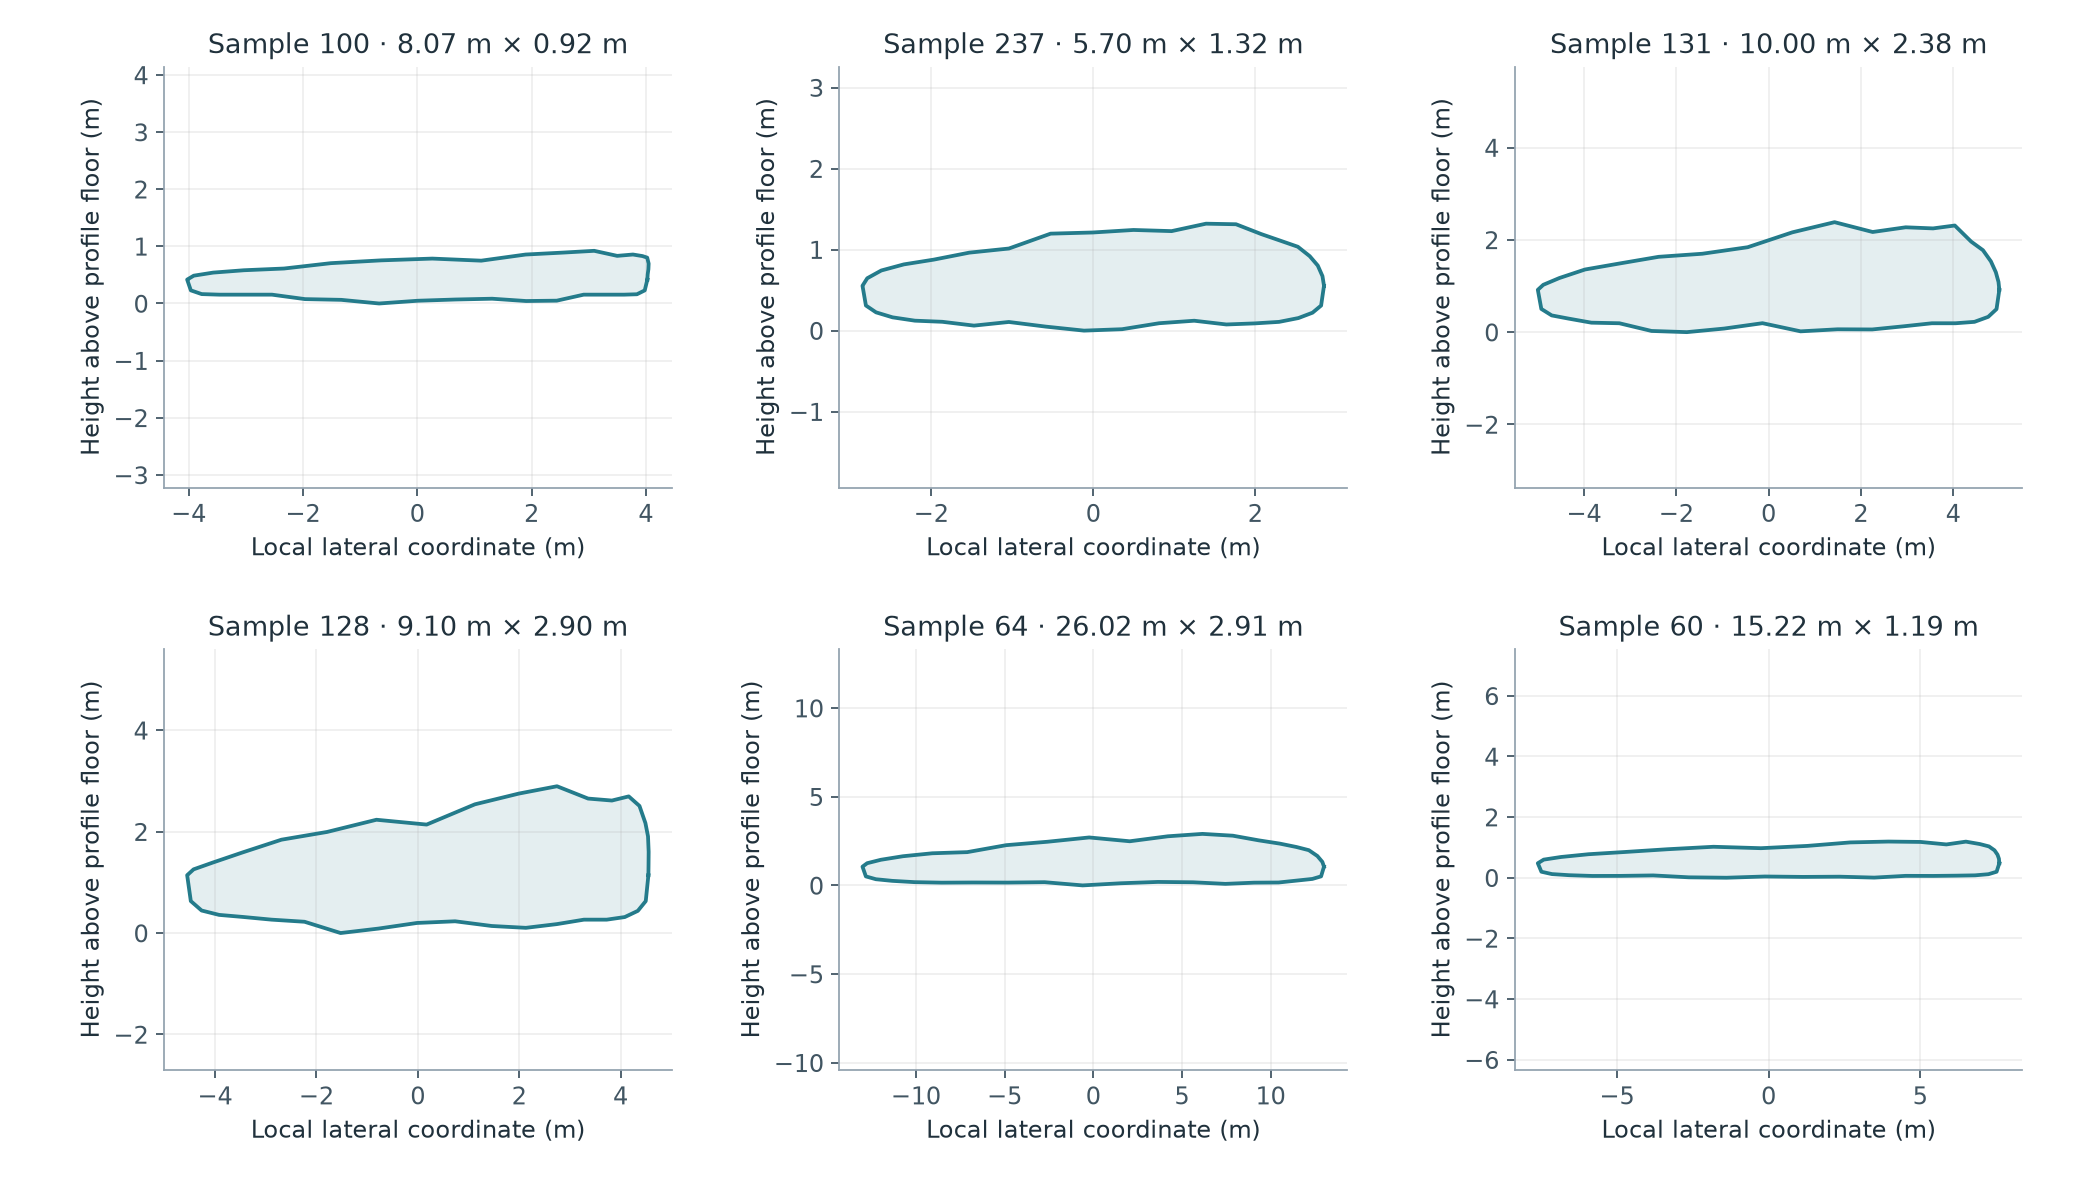
\includegraphics[width=\textwidth,height=105mm,keepaspectratio]{figures/f04_sections.png}
\caption{Six Stage-C section envelopes from the saved Earth inspection scenario, seed 4. Four low-junction samples and two wide locations illustrate variation in aspect ratio, floor shape, and roof profile. Sample IDs and measured envelope dimensions identify the examples. Each panel uses equal metric axes, with different limits; these are selected profiles from one world, not a population-level validation or cuts through the final mesh.}
\label{fig:geometry}
\end{figure*}

\subsection{Geometry-Specific Roof Screening}
\label{sec:roof}
The local roof screen supplements the host-scale routing surrogate (Figure~\ref{fig:roof-screen}). It treats an unsupported roof as a simply supported beam of unit breadth under self-weight. Let $W$ be span, $H$ cavity height, $d_f$ floor depth below the local surface, and $t=d_f-H$ roof thickness. With a strength safety factor $F_s\geq1$, the required roof thickness is
\begin{equation}
t_{\mathrm{req}}=\frac{3F_s\rho gW^2}{4\sigma_{\mathrm{eff}}},\qquad
R_s=\frac{t_{\mathrm{req}}}{\max(t,\epsilon_t)}.
\label{eq:beam}
\end{equation}
The coefficient follows from maximum bending stress under uniform self-weight. A candidate passes the intact-roof screen when $t>0$ and $R_s\leq1$. At a fixed roof thickness, the corresponding width bound is
\begin{equation}
W_{\max}=\sqrt{\frac{4\sigma_{\mathrm{eff}}t}{3F_s\rho g}}.
\label{eq:span}
\end{equation}
At a fixed floor depth, increasing cavity height consumes cover, so $H_{\max}=\max(d_f-t_{\mathrm{req}},0)$ is a conditional bound. It is not a universal maximum tube height for a planetary body.

Stage C evaluates transformed profile elevations, and Stage D reassesses the section envelopes and enlarged junction volumes used for reconstruction. Failed envelopes are represented locally by solid breakdown plugs. These modifications can close passages and can produce an empty accessible result. They are independent of optional debris density and event-route preservation. The graph still records the proposed formation network, while stability records explain the subsequent blockage.

The screen is a conservative procedural construction under restricted assumptions. It omits arching, lateral confinement, regional stress, layering, detailed fracture mechanics, sidewall failure, and support pillars. It samples envelopes and junctions rather than solving the final surface pointwise; later visual smoothing and displacement are outside its mechanical interpretation. Formation dimensions remain separate controls. Equations~\eqref{eq:beam}--\eqref{eq:span} therefore support sensitivity analysis, not a claim that a generated cave is physically stable.

\begin{figure*}[t]
\centering
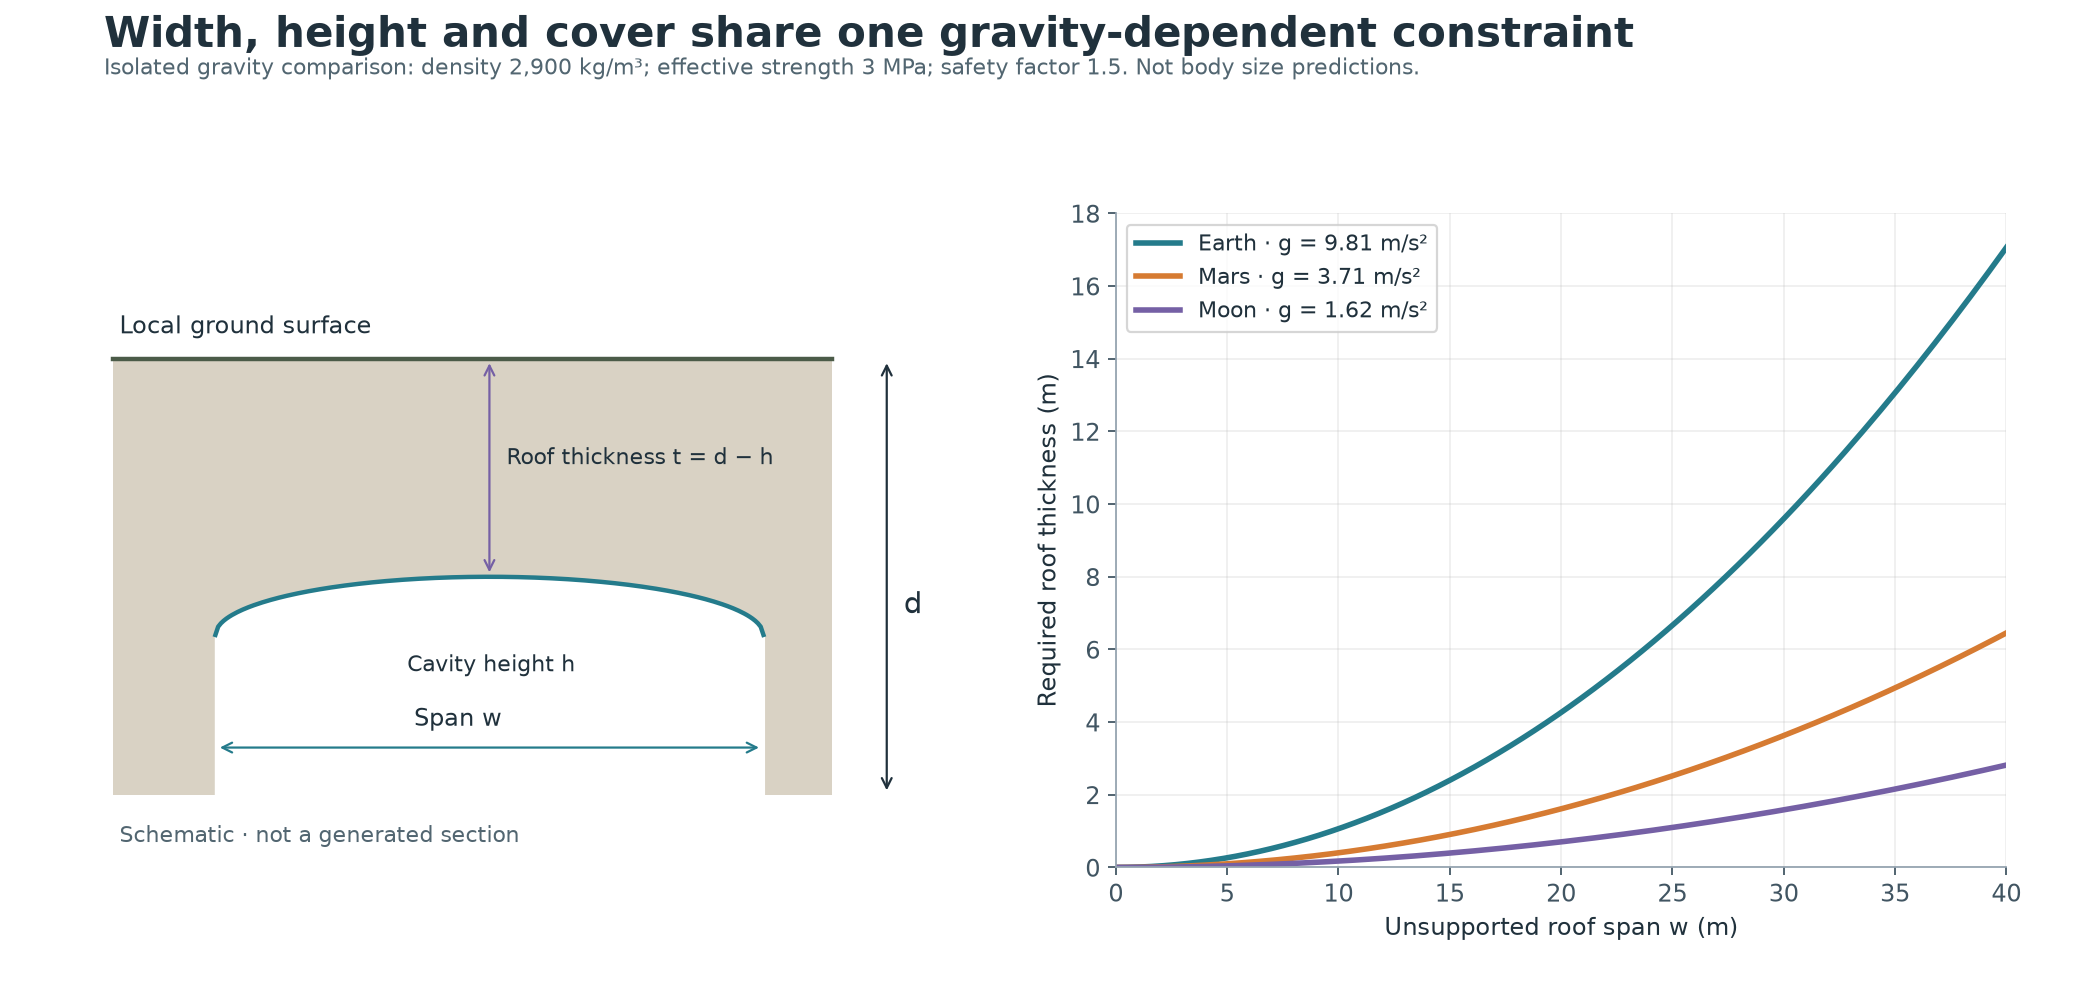
\includegraphics[width=\textwidth,height=86mm,keepaspectratio]{figures/f05_roof_screen.png}
\caption{Geometry of the local roof screen and its isolated gravity sensitivity. The schematic defines span, cavity height, floor depth, and roof thickness; it is not a measured cave cross-section. Curves evaluate Equation~\eqref{eq:beam} with density 2,900 kg/m$^3$, effective strength 3 MPa, and safety factor 1.5. Only gravity changes between curves. The result is a conditional beam-screen requirement, not a prediction of body-specific tube sizes.}
\label{fig:roof-screen}
\end{figure*}

\subsection{Dense and Tiled Volumetric Reconstruction}
Stage D stamps locally oriented conduit primitives from the section field into a scalar density representation. Additional support around connected junctions and chambers bridges the transition between segment semantics and volumetric union. In the implementation's sign convention, values above the isovalue represent cave void and lower values represent solid material. After subtracting the isovalue, a schematic union is
\begin{equation}
\phi_0(\mathbf{x})\simeq\operatorname{smax}_{i}\phi_i(\mathbf{x}),
\qquad \Omega_{\mathrm{void}}=\{\mathbf{x}:\phi(\mathbf{x})>0\},
\label{eq:volume}
\end{equation}
where $\operatorname{smax}$ denotes the configured union or smooth blending operation. The field is density-like; blending and procedural deformation do not guarantee an exact signed-distance function. The zero set is polygonized using marching-cubes reconstruction \cite{marching1987}.

For a bounding box of dimensions $L_x,L_y,L_z$ and voxel spacing $h_v$, dense storage requires approximately
\begin{equation}
N_{\mathrm{dense}}\simeq
\prod_{a\in\{x,y,z\}}\left(\left\lceil L_a/h_v\right\rceil+1\right)
\label{eq:dense}
\end{equation}
samples. This cubic dependence on resolution becomes expensive when a long, narrow network occupies a small fraction of its box. Tiled storage allocates active spatial regions around the conduits and modifiers, with neighboring samples available for boundary processing. For $N_t$ active tiles of side $b$ samples and halo width $r$, density storage is of order $N_t(b+2r)^3$, with additional costs for metadata and temporary arrays.

Tiling reduces empty-space storage; it does not guarantee bounded total memory independent of cave size. Surface extraction, global vertex welding, material preparation, and export can still require substantial memory. The final surface is assembled across processing chunks to remove duplicate boundary vertices and support continuous visual normals. Collision geometry is prepared separately so its complexity can be controlled independently of the visual mesh.

Resolution must be reported relative to the features being represented. A nominally narrow passage may disappear if its clearance approaches the voxel spacing; a small rock can be below the grid scale even when its separate prop mesh is detailed. Wider chamber unions may also change topology relative to the graph. Mesh continuity, connected components, preserved passages, and local section cuts therefore complement triangle count as reconstruction diagnostics.

\subsection{Structural Events and Grounded Debris}
Stage E constructs static hazard scenarios after a queryable cave volume exists. Collapse, choke, and infill modifiers add solid material within the cave and alter the final density boundary. With a signed obstacle-exterior field $\psi_k$ that is positive outside obstacle $k$, the corresponding schematic operation is
\begin{equation}
\phi_{k+1}(\mathbf{x})\simeq
\operatorname{smin}\bigl(\phi_k(\mathbf{x}),\psi_k(\mathbf{x})\bigr).
\label{eq:events}
\end{equation}
The final meshing pass therefore includes these changes in the wall and collision boundary. By contrast, loose rocks and boulders remain separate scene objects with their own geometry and event metadata.

Figure~\ref{fig:events} illustrates event placement and per-realization diagnostics. Candidate ranking can use structural controls together with inherited temperature, age, flux, and maturity. Cooler, mature, or lower-flux reaches can receive increased procedural deposition preference. Prop placement queries the actual base surface, aligns objects to inward floor normals, and embeds them slightly to avoid floating. Collapse-associated clusters retain parent-event identity. Placement reports expose accepted and rejected candidates rather than assuming every requested prop was successfully placed.

An optional preservation mode checks local bypass or clearance conditions when applying the configurable events. It may reduce or reject an event that violates the specified condition. This is a scenario-selection rule for experiments requiring a usable route, not a geological formation law or a general robot-feasibility proof. The independent roof-screen plugs are not undone by that mode. Studies using it should report the setting because rejection conditions the distribution of accepted hazards.

\begin{figure*}[t]
\centering
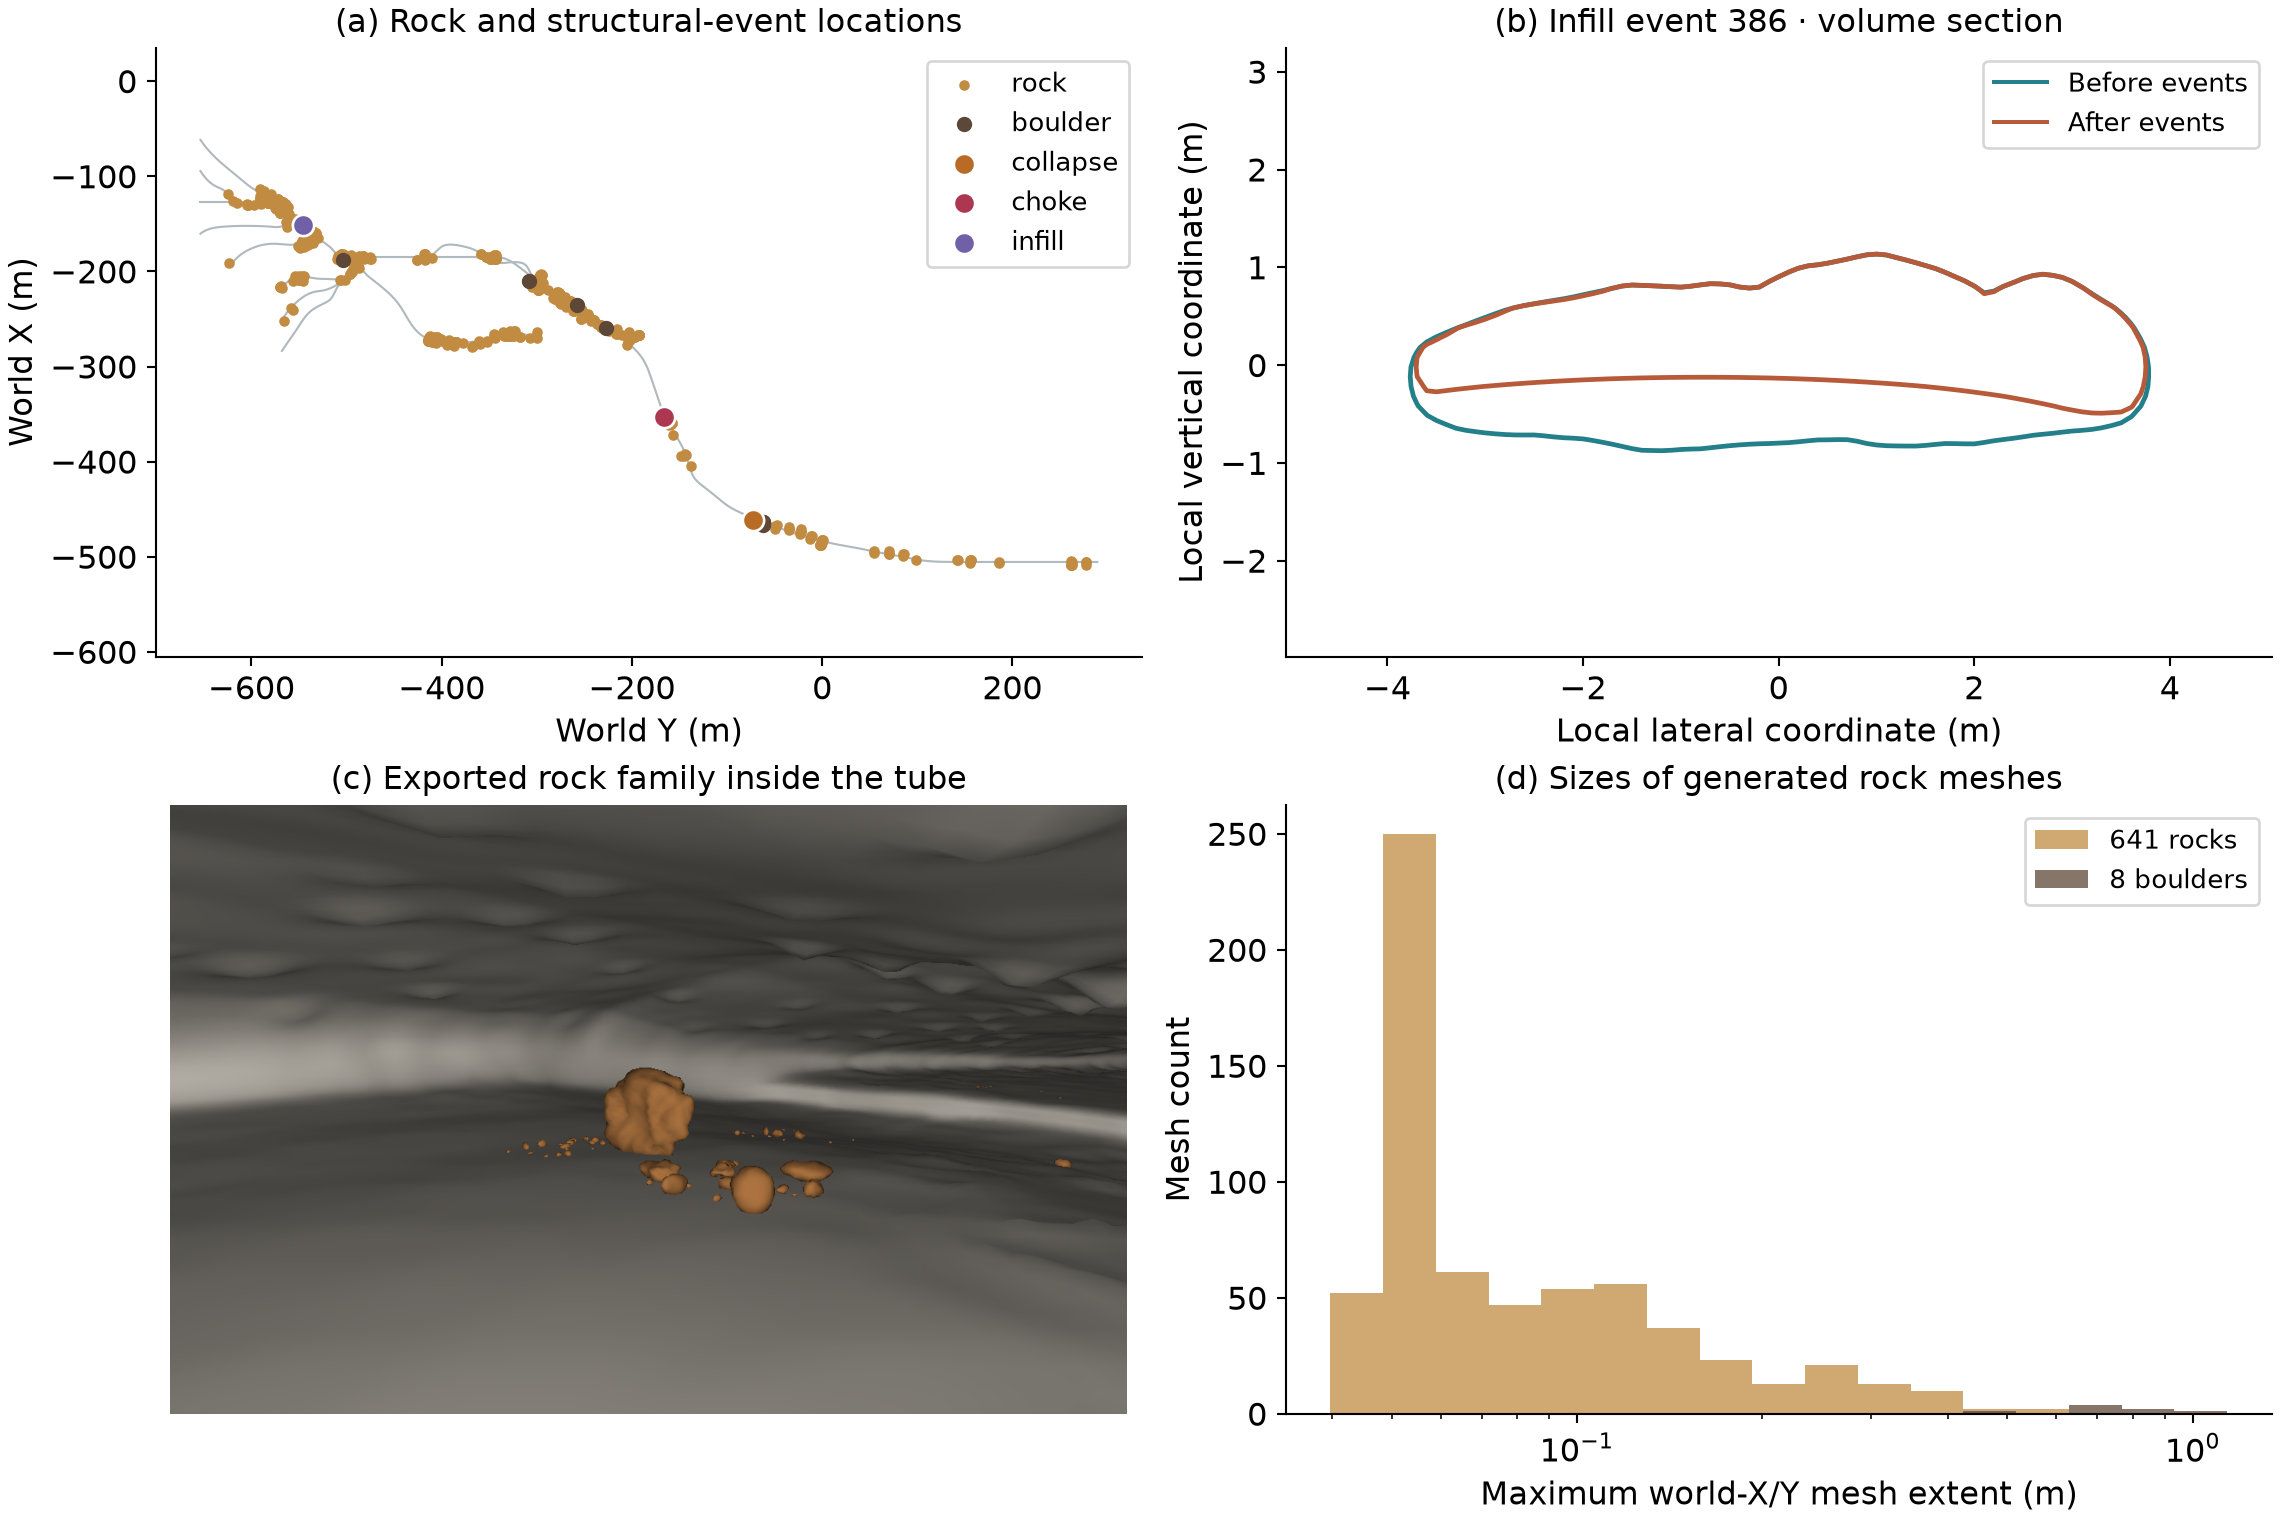
\includegraphics[width=\textwidth,height=112mm,keepaspectratio]{figures/f06_events.png}
\caption{Current Earth seed-4 event scenario at 0.20 m voxel spacing, with 641 rocks and eight boulders generated by Rocky and exported as 649 separate meshes. (a) Prop and structural-event locations. (b) Before/after volume contours at infill event 386; one choke and one infill modifier were applied, while the collapse modifier was rejected by the volume safeguards. (c) An interior view of the exported scene, with ochre identifying rock props and gray identifying the cave under diagnostic lighting. (d) Actual rock-mesh dimensions in world coordinates. This is one development scenario, not a confirmatory campaign; the original no-event inspection GLB is preserved.}
\label{fig:events}
\end{figure*}

\subsection{Intrinsic Floor Atlas and Post-Event Refresh}
\label{sec:atlas}
A single height value indexed by $(x,y)$ cannot distinguish floors in vertically overlapping passages. The authoritative floor atlas instead uses intrinsic coordinates
\begin{equation}
\mathbf{u}=(e,s,\ell),
\label{eq:intrinsic}
\end{equation}
where $e$ identifies a segment, $s$ is longitudinal distance, and $\ell$ is lateral offset in its local frame. Each sample additionally stores world position, vertical level, inward normal, clearance, and grounding status. Segment bands provide a convenient atlas visualization, while plan coordinates remain available as a nonunique preview.

Floor candidates are lifted to the density boundary and checked for clearance. After structural events, surviving candidates are queried again, and invalidated cells are recorded. Figure~\ref{fig:atlas} illustrates the retained floor information. The refreshed atlas can carry geology labels and event influence, including sediment, breakdown, debris, and constriction information. A field computed against the pre-event floor must not be presented as the post-event traversable surface.

The atlas is a set of local charts rather than a globally unique geometric parameterization. Adjacent segment charts can overlap around junctions, so cross-chart adjacency must use graph semantics and world-space geometry. Segment identity disambiguates stacked passages but does not itself define a path planner. Nor is pointwise overhead clearance sufficient for a robot's swept volume: body width, turning radius, floor slope, gaps, and contact geometry remain relevant.

Loose props require an additional distinction. Floor lifting and structural clearance refer to the queried cave density. Separate rocks and boulders participate in the scene as objects and are not automatically equivalent to solid voxels in that field. A downstream traversability map must combine the atlas with the final collision scene, including those props, rather than use atlas clearance alone as a collision guarantee.

\begin{figure*}[t]
\centering
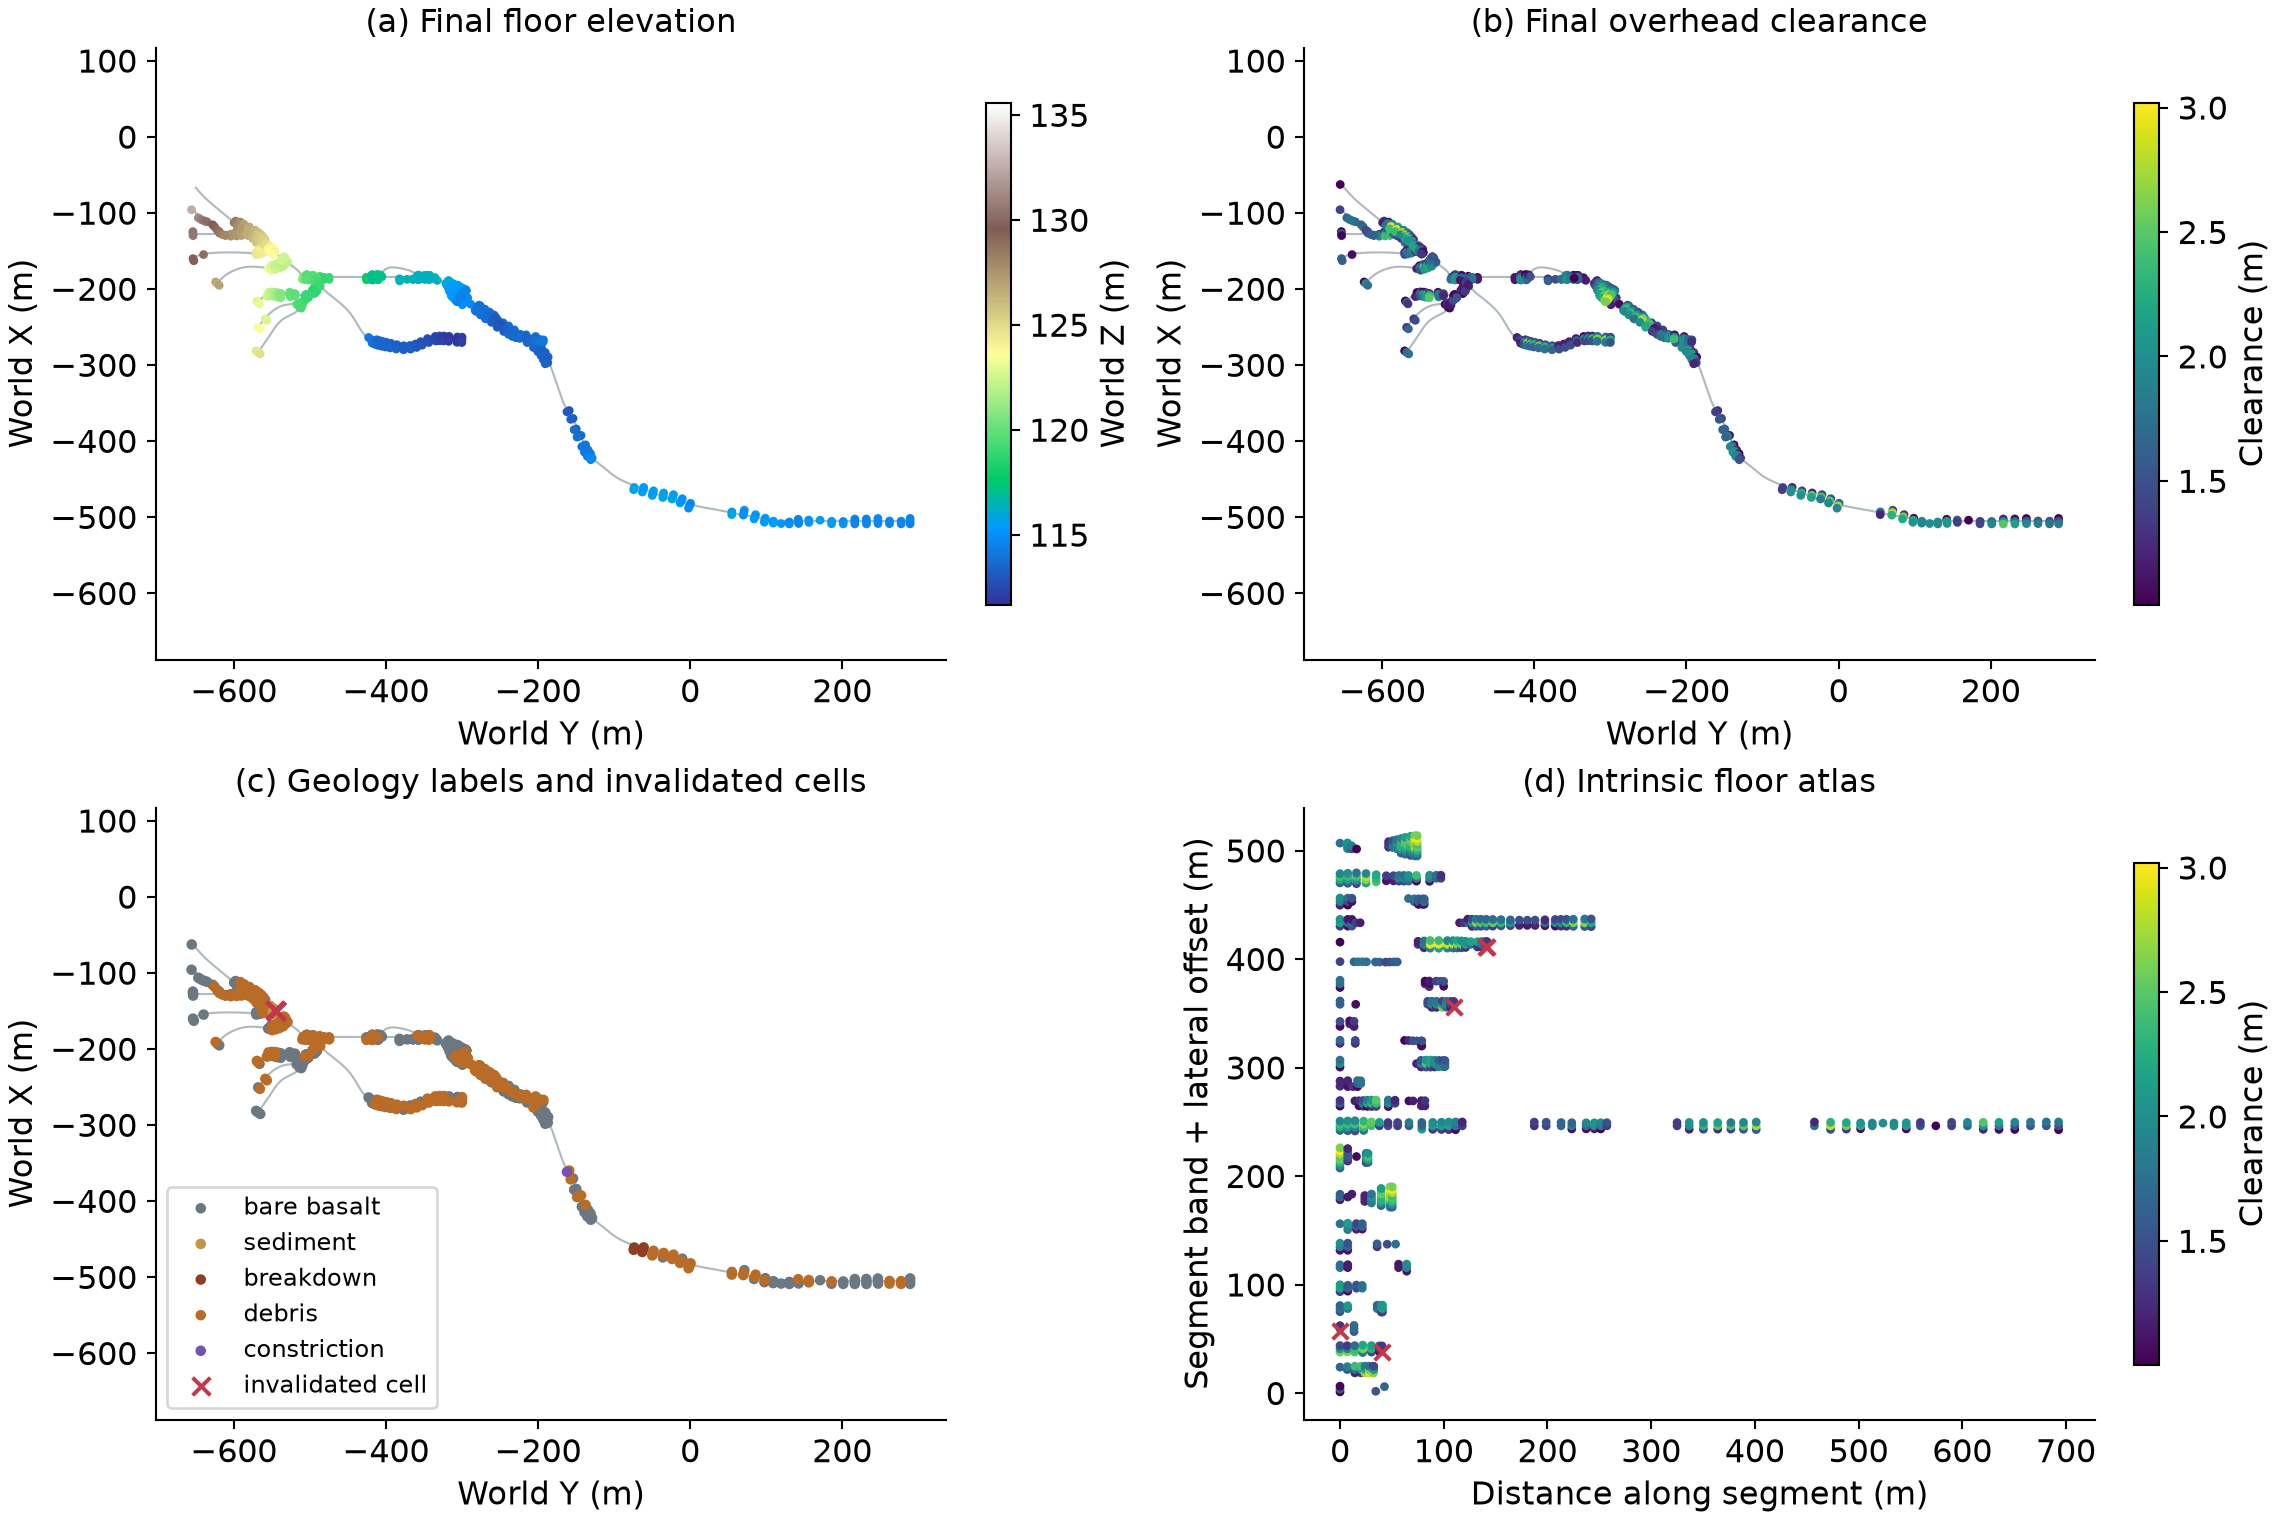
\includegraphics[width=\textwidth,height=122mm,keepaspectratio]{figures/f07_floor_atlas.png}
\caption{Floor atlas refreshed for the rock-enabled seed-4 scenario in Figure~\ref{fig:events}. The base atlas has 635 cells; relifting retains 630 across 25 segment bands and invalidates five, shown as crosses. Panels show final elevation, overhead clearance, procedural geology labels, and intrinsic coordinates. Cells require at least 1 m overhead clearance at 0.20 m voxel spacing. Clearances query the cave volume; the 649 separate rock meshes must also be considered for collision and traversability. Breakdown coloring retains collapse-influence metadata even though that volume modifier was rejected. Counts describe this realization only.}
\label{fig:atlas}
\end{figure*}

\subsection{Canonical Scene, Appearance, and Export}
The final scene separates visual appearance from physical collision. Surface preparation includes smoothing, UV charts, metric texture scaling, seam-consistent visual displacement, and normal/tangent recomputation. The collision surface can retain the undisplaced geometric boundary. This distinction allows stable collision preparation while supporting richer appearance, but it also creates a measurable visual-to-collision offset that should be considered for close-range contact or perception experiments.

The current portable appearance path packages physically based rendering channels and prepares geometry for their use. It does not yet implement a complete geology-conditioned material synthesis model, explicit visual levels of detail, or a finite outer rock shell. The cave wall is an inward-facing void boundary. Exterior inspection may therefore require a cutaway or an appropriate diagnostic rendering mode rather than implying a watertight solid rock mass.

Adapters package the canonical scene for Blender, Unreal Engine, Unity, Gazebo, and Omniverse using the supported interchange or native scene formats. Axis, handedness, and unit conventions belong to the adapter; generation is not rerun for each target. Manifests connect visual assets, separate collision geometry, material dependencies, and provenance. Export availability establishes an implementation capability, while successful import and physical scale require separate checks in the receiving applications.

For a point $\mathbf{x}$ in canonical coordinates, a target transform can be written
\begin{equation}
\mathbf{x}_k=a_kR_k\mathbf{x}+\mathbf{t}_k,
\label{eq:transform}
\end{equation}
where $a_k$ is the unit scale and $R_k$ includes the axis convention, possibly with a handedness change. Comparisons use the inverse transform to return imported assets to canonical coordinates. This avoids mistaking a coordinate permutation for a scale error. Identical underlying geometry does not imply identical illumination, sensor noise, material response, or contact dynamics across engines.

A saved controlled-reach study also illustrates optional geometry-stage surface relief (Figure~\ref{fig:surface-relief}). In that study, wall, roof, and floor accretion modify the density before the roof screen and final meshing. The depicted relief is geometric and is distinct from the visual texture displacement described above. The isolated reach has artificial closed ends and is used here to illustrate surface construction, not as a complete cave or a confirmatory validation case.

\begin{figure*}[t]
\centering
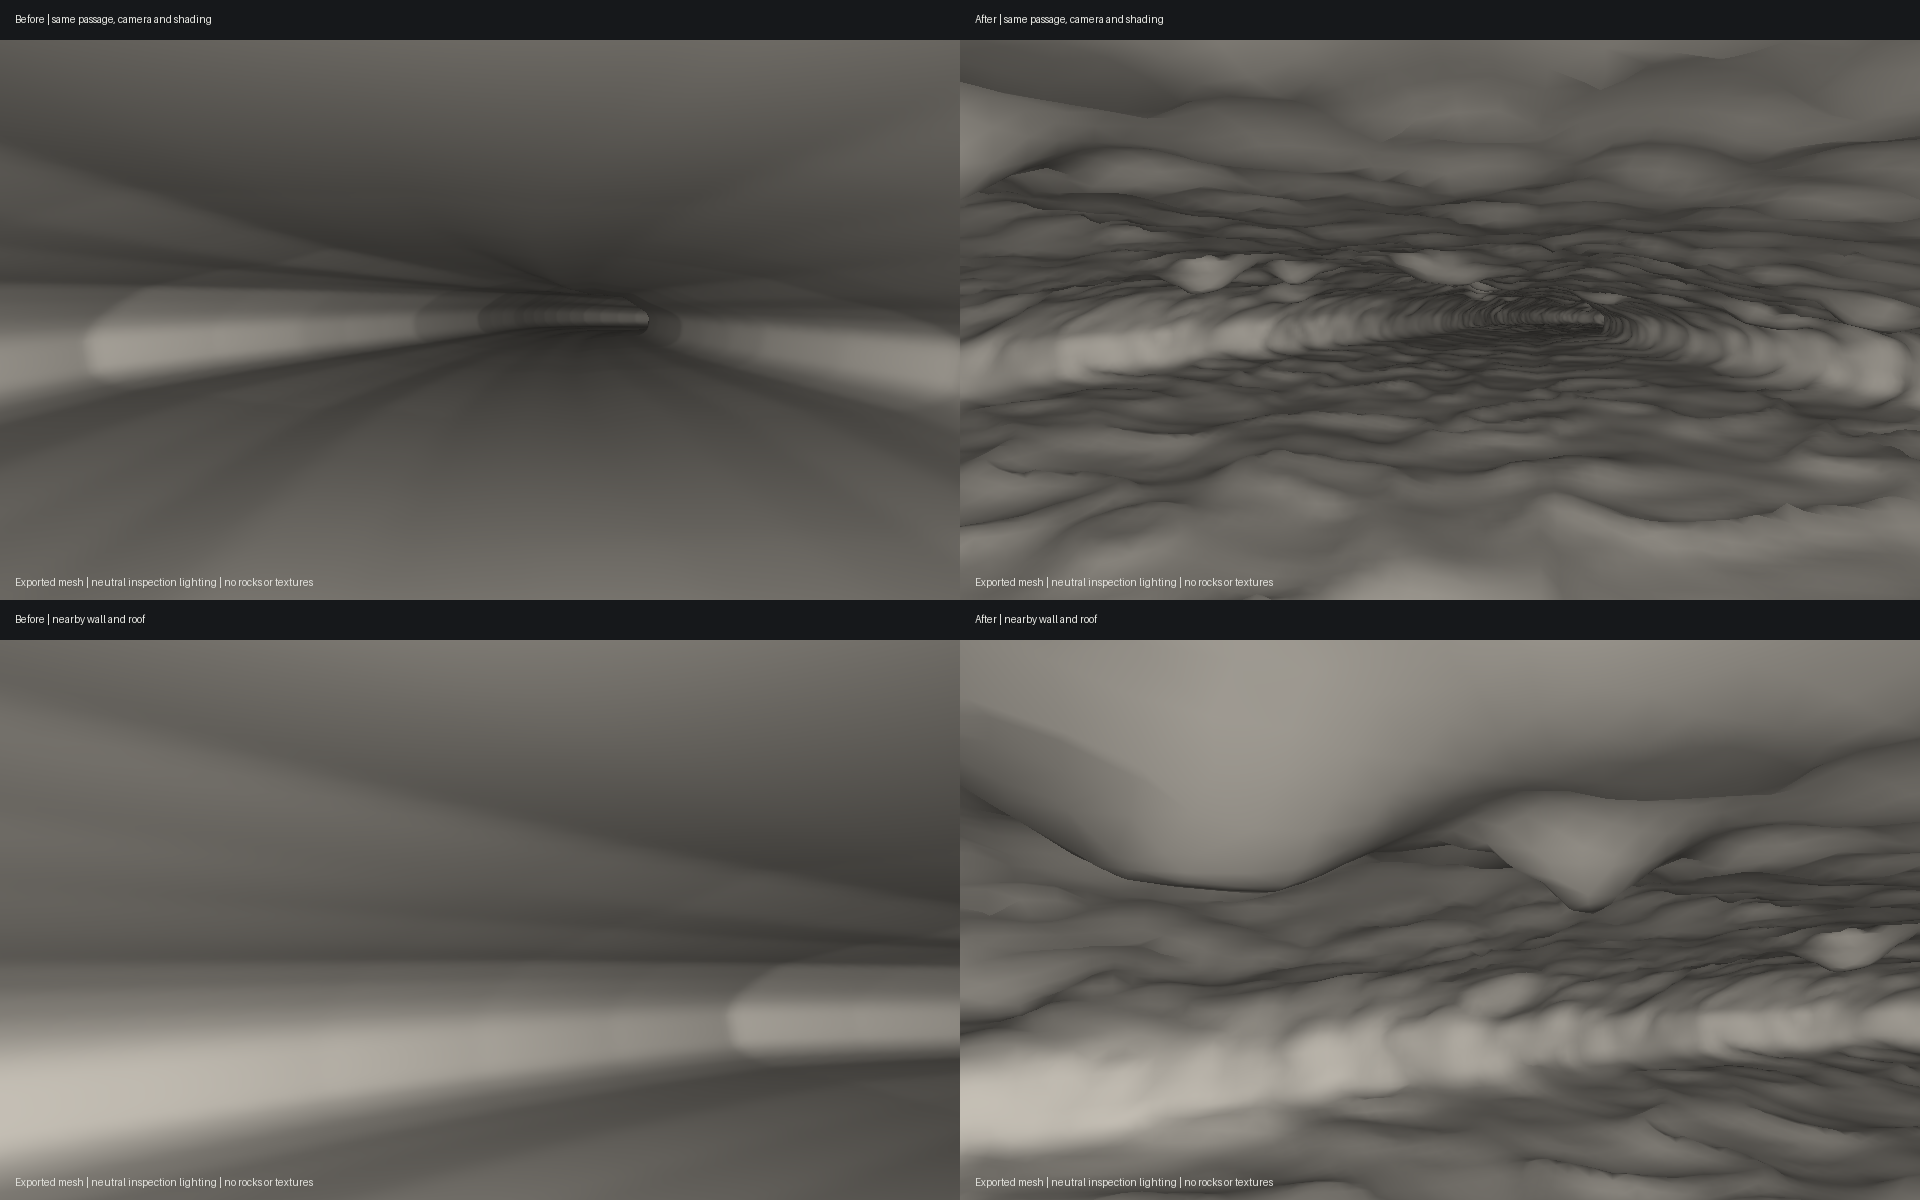
\includegraphics[width=\textwidth,height=108mm,keepaspectratio]{figures/f08_surface_relief.png}
\caption{Surface-relief illustration from a saved isolated-reach development study. Left and right columns show the same passage before and after geometric accretion, using matched camera and shading settings. The upper row looks along the passage; the lower row inspects the nearby wall and roof. Neutral inspection lighting is used without rocks or textures. The far closure belongs to the isolated test reach. This comparison is separate from the seed-4 network and the confirmatory experiments.}
\label{fig:surface-relief}
\end{figure*}

\section{Experimental Methodology}
\label{sec:experiments}
The evaluation separates implementation properties, empirical morphology, and robotics relevance. RQ1 asks whether terrestrial profiles agree with selected reference descriptors. RQ2 asks whether parameter and routing-term interventions measurably affect the generated environment. RQ3 asks how adaptive sampling changes geometric fidelity at a comparable sample budget. RQ4 asks how computational cost scales and whether exported assets preserve canonical scale and content. Determinism and artifact provenance support all four questions.

\begin{table*}[t]
\caption{Declared experiment settings in the current evaluation configuration. Counts describe planned seeds or conditions, not completed measurements.}
\label{tab:campaign}
\centering\small
\begin{tabularx}{\textwidth}{@{}p{2.65cm}p{2.2cm}YY@{}}
\toprule
Experiment & Seed count & Declared comparison & Principal outputs \\
\midrule
Terrestrial morphometry & 100 & PDC confirmatory partition; generated profiles; width/height-matched ellipses & Per-descriptor normalized Wasserstein distance, KS statistic, clustered intervals \\
Controllability & 100 & Three levels each of distributary tendency, duration, inflation, and supply & Paired topology, extent, and geometry responses \\
Routing-term ablation & 100 & Full; five single-term removals; constant routing cost & Route displacement, term exposure, split/merge and cycle-rank changes \\
Section sampling & 30 & Adaptive; approximately count-matched uniform; 1 m reference spacing & Actual counts; symmetric mean and 95th-percentile point errors \\
Scalability & 5 & 0.5, 1, 2, 5 km requested routes; dense and tiled; standard quality & Wall time, peak RSS, realized geometry and completion status \\
Export consistency & 3 & Blender, UE5, Unity, Gazebo, Omniverse packages & Canonical identity, bounds, geometry and collision checks \\
Determinism & 3 & Repeats and downstream interventions & Semantic hashes and expected invariants \\
\bottomrule
\end{tabularx}
\end{table*}

\subsection{Frozen Configuration and Provenance}
Table~\ref{tab:campaign} summarizes the declared campaign. A run is identified by its seed, resolved configuration, generator revision, dependency versions, schema versions, and input hashes. The current seed lists contain 100 network seeds, 30 sampling seeds, five geometry seeds, and three export/determinism seeds. Bootstrap settings declare 2,000 iterations and 95\% confidence intervals. Completion counts and failures are reported separately from these declared denominators.

The evaluation uses persistent case records and saved stage artifacts. Reuse is valid only when the case fingerprint matches; obsolete attempts are archived. Failed, invalid, and timed-out cases remain visible in campaign denominators. Measured result figures and generated tables consume saved results rather than silently triggering new generation. The illustrations included here are identified separately as schematics or saved development/documentation artifacts. For this campaign, the actual modified package, project configuration, seed lists and partition files were copied before evaluation to a dated source snapshot. The snapshot file manifest and executing-package hash identify the uncommitted implementation; the base commit alone is insufficient. The source is loaded from a preserved snapshot throughout execution. Before the controllability sweep began, a separately recorded evaluator amendment replaced outdated partial edits of derived settings with full project-configuration resolution. All 12 control settings matched literal TOML edits in tests; default resolved configuration hashes were identical between revisions. The other six experiments retain their original snapshot. This correction did not fit any generator parameter to evaluation results. Texture assets are referenced separately with content hashes.

The workstation has an Intel Core i5-12400F (six physical cores, 12 logical CPUs), 31.2 GiB RAM, Linux 6.8 and Python 3.13.5. Numerical-library thread counts are fixed at one. Independent non-benchmark cases use four processes, or six for the amended controllability sweep; resource benchmarks use one child at a time. This is a shared workstation, not a guarantee of an otherwise idle machine. Dependency versions and optional backends are recorded in the campaign provenance. Manual import records additionally identify the receiving application's version. A short development pilot is useful for checking instrumentation, but its sample count and status must remain distinct from the final campaign.

\subsection{Reference Data, Partitioning, and Sampling Bias}
The terrestrial reference is PDC version 2.0, pinned to the version-specific Zenodo record \cite{pdc2025}. The public release describes more than 1,200 sections from more than 94 tubes; the repository's audited identifier inventory contains 95 caves. Exact usable section counts depend on the parser and validity rules and must be reported from the campaign inventory.

The existing split partitions 76 cave identifiers for calibration and 19 for confirmatory evaluation. Identifiers were ranked by a deterministic hash of a frozen salt and cave ID; morphology was not used to allocate caves. All sections from a cave remain in one partition. An exploratory whole-catalog summary existed before this split was created, so the confirmatory partition is not described as historically unseen. From the split freeze onward, parameter selection is restricted to the calibration partition. Any later inspection used for tuning must be disclosed and would change the interpretation of the confirmatory evaluation.

Contour auditing preserves the documented vertical direction and checks finite coordinates, sufficient unique vertices, nonzero dimensions, valid area, and the declared exclusion of self-intersections. Rejected records retain their cave identity and reason. Duplicate endpoints and contour orientation are normalized consistently without repairing invalid shapes in a way that silently changes morphology.

Reference sections are neither independent samples nor a uniform survey of all lava tubes. Some caves have many more sections, survey locations may emphasize accessible or distinctive regions, and digitization resolution varies. The primary pooled descriptor comparison is therefore section-weighted. Cluster resampling addresses dependence but does not make every cave equally weighted. A cave-balanced sensitivity analysis is desirable as a separately declared extension. Generated adaptive samples are also denser around curvature and junctions; an equal-arc-length resampling sensitivity would assess this additional representation bias.

\subsection{Morphometric Descriptors and Baselines}
For each valid contour, we compute width $W$, height $H$, aspect ratio $W/H$, area $A$, perimeter $P$, and compactness
\begin{equation}
Q=\frac{4\pi A}{P^2}.
\label{eq:compactness}
\end{equation}
Two additional implemented descriptors quantify floor residual and roof asymmetry. Let $\mathcal{L}$ contain boundary vertices within the lowest 20\% of section height, and fit $\widehat{v}(u)=au+b$ by least squares. The floor residual is
\begin{equation}
F_{\mathrm{floor}}=\frac{1}{H}
\sqrt{\frac{1}{|\mathcal{L}|}\sum_{i\in\mathcal{L}}
\bigl(v_i-\widehat{v}(u_i)\bigr)^2}.
\label{eq:floor-metric}
\end{equation}
Let $\mathcal{U}$ contain the boundary vertices in the upper half of section height and $u_c$ denote the polygon-centroid horizontal coordinate. Roof asymmetry is
\begin{equation}
R_{\mathrm{roof}}=\frac{|\operatorname{mean}_{i\in\mathcal{U}}u_i-u_c|}{W}.
\label{eq:roof-metric}
\end{equation}
These are operational descriptors, not unique geological definitions. Both depend on how the boundary is sampled. A low floor residual indicates closeness to a fitted line in the selected lower band; it is not equivalent to robot traversability or a level floor.

For a descriptor with reference distribution $P_r$ and generated distribution $P_g$, normalized one-dimensional Wasserstein distance is
\begin{equation}
\widetilde{W}_1(P_r,P_g)=
\frac{W_1(P_r,P_g)}{\max(\operatorname{IQR}(P_r),\epsilon_m)}.
\label{eq:normalized-w1}
\end{equation}
The safeguard $\epsilon_m$ uses the descriptor's numerical units. Descriptors with near-zero reference IQR should be flagged because normalization can amplify small differences. The two-sample Kolmogorov--Smirnov statistic describes the largest ECDF separation; ordinary independent-sample $p$-values are not used to establish significance for correlated cave sections.

The baseline is an ellipse constructed with the width and height of each generated section. It therefore has the same generated width, height, and aspect-ratio distribution by construction. Differences in compactness, floor residual, and asymmetry test the added shape controls. The baseline does not test whether PLUME-Advanced samples size better, nor does it substitute for running the original PLUME or Pyroduct software. The predeclared aggregate averages normalized distances for aspect ratio, compactness, floor residual, and roof asymmetry. Since aspect ratio is identical between the matched baseline and generated profiles, that term cannot explain their difference.

Uncertainty is estimated by resampling reference cave IDs and generated world IDs as independent clusters, retaining all selected sections within each sampled cluster. Per-descriptor intervals accompany distance estimates. The aggregate interval uses the same cave/world draws across its four descriptors: each bootstrap replicate averages the four recomputed distances. Cached sorted distributions and integer cluster multiplicities evaluate exactly the empirical distances and linearly interpolated reference quartiles of the repeated samples; interval endpoints are not averaged. The primary experiment stops at Stage C: it assesses the generated section prior. Separate cuts through the final mesh are needed to show that volumetric reconstruction, structural plugs, and events preserve or change those descriptors as intended.



\subsection{Parameter Interventions and Routing-Term Ablations}
The declared controllability sweep uses distributary values $\{0.20,0.50,0.80\}$, duration multipliers $\{0.50,1.00,1.50\}$, inflation values $\{0.20,0.50,0.80\}$, and supply multipliers $\{0.70,1.00,1.30\}$. One family changes at a time with matched seeds. These controls are interpreted through their resolved parameters: for example, a supply change may alter host scale as well as network properties. Fixed seed pairing reduces stochastic variation but does not promise point-for-point graph correspondence after a structural change.

The declared primary readouts are cycle rank for distributary tendency, main-route length for duration, junction-to-passage width ratio for inflation, and resolved host horizontal scale for supply. The last is an input-resolution check rather than an independent observation of generated geometry. Supplementary paired summaries compare the highest and lowest declared levels using the same median-difference bootstrap estimator.

Network descriptors include total centerline length, node and edge counts, split and merge counts, chambers, branch persistence, terminal structure, route sinuosity, and vertical levels. The undirected cycle rank is
\begin{equation}
\beta_1=|E|-|V|+c,
\label{eq:cycles}
\end{equation}
where $c$ is the number of connected components and the counting convention retains relevant parallel edges. This measures independent alternatives in the formation graph. A directed acyclic braid can have $\beta_1>0$.

The routing experiment includes the full model, five single-term removals, and a constant-cost condition. Remaining weights are normalized consistently with Equation~\eqref{eq:routing}. Terrain guidance and downstream consumers of the host remain present in the constant-cost case; ``unconditioned'' in existing result filenames means routing-cost conditioning is disabled, not that every host influence has been eliminated.

Route comparisons should include geometry and exposure as well as graph counts. A network can move away from a fractured region without changing its number of branches. Symmetric centerline displacement captures movement when segment identities differ, while cost-term exposure indicates whether routes occupy different host conditions. For a metric $m$, paired changes are $\Delta m_i=m_i^{\mathrm{intervention}}-m_i^{\mathrm{full}}$. Median changes and paired confidence intervals preserve the seed pairing. Nonresponse, direction reversals, saturation, and failed cases are reported, rather than assumed to agree with the intended control semantics.

\subsection{Adaptive Sampling Fidelity}
The implemented sampling ablation compares adaptive sections against an approximately count-matched uniform policy on the same network. A dense reference uses 1 m longitudinal spacing. If the adaptive policy produces $N_a$ samples over $n_e$ segments of total length $L$, the uniform spacing is initialized near $L/(N_a-n_e)$. Endpoint rounding changes actual counts, which must be reported instead of claiming exact budget equality.

The current metric constructs world-space point clouds from the sampled profile boundaries. Let $X$ and $Y$ be candidate and reference points, and $d(\mathbf{x},Y)=\min_{\mathbf{y}\in Y}\|\mathbf{x}-\mathbf{y}\|_2$. The pooled bidirectional mean is
\begin{equation}
E_{\mathrm{pts}}=
\frac{\sum_{\mathbf{x}\in X}d(\mathbf{x},Y)+
\sum_{\mathbf{y}\in Y}d(\mathbf{y},X)}{|X|+|Y|}.
\label{eq:error}
\end{equation}
The 95th percentile of the pooled distances complements the mean. This is a sampled point-set discrepancy, not an exact distance between continuous surfaces, a Hausdorff bound, or a final mesh error. It is sensitive to sample placement and density. A stronger claim of fewer sections at matched geometric error requires a spacing sweep and a common error target; timing savings also require dedicated Stage-C timing. Those claims are not implied by the current count-matched experiment.



\subsection{Scalability and Reconstruction Diagnostics}
Dense and tiled storage are compared at requested route lengths of 0.5, 1, 2, and 5 km under the declared standard-quality configuration. Each benchmark runs in a separate child process with a declared 7,200 s timeout and a monitored 12 GiB process-tree RSS limit, sampled every 0.05 s. Benchmark cases run sequentially on the shared workstation, after other campaign workers have exited. Process-tree startup and teardown are included in wall time. Record both requested and realized route length: the stochastic network, branches, and body resolution may cause them to differ. Report voxel spacing, realized width range, active tile or voxel count, triangle count, and surviving free-space components alongside wall time and peak resident set size.

The measured path generates host fields, network, sections, base density with roof screening, and the finalized mesh including welding. It excludes optional geological events and rock props, appearance preparation, asset packaging, and application import. Standard Earth resolution is 0.6 m; this is coarser than the separate 0.2 m illustrative inspection scene. The recorded count of input profiles with fewer than eight voxels across their smallest dimension is a resolution warning, not a convergence test. These resource measurements cannot support an end-to-end or high-fidelity timing claim. Export size is reported for a clearly defined package. Failed or timed-out dense cases remain in the plot or table; they are not assigned a made-up speedup. Where both modes complete, compare paired cost together with geometry fidelity so that a faster but less faithful reconstruction is not treated as an equivalent result.

Local section cuts and continuity diagnostics test for unintended closures, accidental passage unions, seam cracks, disconnected surfaces, and under-resolved morphology. A small numerical difference in bounds alone cannot certify unchanged topology. Roof-screen failures should be separated from meshing failures, because the former may be an intended outcome of the procedural structural constraint.

\subsection{Portability and Determinism Checks}
The automatic export experiment checks the emitted visual and collision assets from three development-size Earth worlds, using the same canonical cave geometry for five target adapters. Optional events and rock props are outside this experiment. Package checks and reported bounds diagnostics must be distinguished from the more extensive material, pose and contact checks below. The automatic bounds diagnostic compares sorted extent vectors using the maximum componentwise relative difference for parsed GLB/OBJ primary files; it does not follow Gazebo package references, apply an inverse pose transform or parse USD bounds. These extents compare the assembled base mesh with the emitted visual surface, which can include shared smoothing and texture displacement. A nonzero difference therefore does not isolate an exporter-transform error. This is not the manual metric in (\ref{eq:bbox}). Application imports follow a separate manual protocol. For every imported target, record version, seed, configuration hash, import transform, screenshots, and pass/fail details. A one-metre reference object tests scale, while a dynamic test object checks contact with the imported collision floor.

After transforming an imported asset back into the canonical frame, bounding-box consistency is
\begin{equation}
\epsilon_{\mathrm{bbox},k}=
\frac{\left\|\mathbf{d}(T_k^{-1}\mathcal{A}_k)-\mathbf{d}(\mathcal{A})\right\|_2}
{\max(\left\|\mathbf{d}(\mathcal{A})\right\|_2,\epsilon_d)}.
\label{eq:bbox}
\end{equation}
Here $\mathbf{d}$ is the three-dimensional extent vector, $T_k$ the complete target transform, and $\epsilon_d$ a positive length safeguard. Translation and orientation require separate landmark or reference-object checks because identical extents do not establish pose. Matching bounds also cannot reveal missing interior surfaces; geometry content and collision checks remain necessary.

The implemented determinism experiment uses three development-size worlds, repeats generation through Stage C, checks checkpoint round trips, and perturbs downstream event and export settings. It compares semantic hashes of A--C artifacts; it does not measure final-mesh or container-byte repeatability. The expected unchanged artifacts must be named in advance. Event and exporter setting changes should preserve A--C in the implemented check. Preservation of the final canonical mesh under exporter changes would require an additional test. Byte-for-byte equality of container files is a separate property because metadata and serialization can vary. No claim of identical sensor rendering or physics is inferred from either package equality or successful import.



\section{Results}
\label{sec:results}
The campaign attempted all 2,076 declared cases across seven experiments. Of these, 2,071 completed and five reached the monitored memory limit. Case completion records that an experiment ran; it does not imply that a scientific hypothesis or every quality criterion was supported. The following results include the observed failures and negative findings.

\subsection{Morphometric Agreement}
Table~\ref{tab:morph} compares 118,257 profiles from all 100 completed Earth worlds with 200 valid contours from the 19 evaluation caves. No selected reference contours or generated worlds were rejected. These are section-weighted distributions; the 118,257 profiles are not independent experimental replicates. The frozen executing package has SHA-256 prefix \texttt{d8bea8ed20c1}; its complete sources and configuration are preserved with the campaign.

The selected aggregate is 0.254 (95\% interval [0.227, 0.417]), versus 0.840 for dimension-matched ellipses, a descriptive reduction of 69.8\%. The largest differences from the ellipse occur in floor residual and roof asymmetry, followed by compactness. This point-estimate reduction is not an interval for the difference between methods. Width, height and aspect ratio have identical distances for both methods by construction.

Figure~\ref{fig:morph-evaluation} shows that absolute dimensions and variability remain mismatched. Generated median width is 8.16 m, versus 5.97 m in the reference, and median height is 4.64 m, versus 3.50 m. Generated width IQR is 2.41 m, compared with 7.90 m in the reference; median area is 27.52 versus 13.95 m$^2$. Thus improved nonelliptical shape descriptors do not establish a calibrated size distribution. This campaign uses the frozen full-route project configuration, distinct from the smaller illustrative inspection scenario. No generator parameters were retuned after these measurements.

\begin{table}[t]
\caption{Terrestrial Stage-C morphology on the evaluation partition: normalized $W_1$ (lower is better). Intervals are for Advanced and use joint cave/world resampling; the aggregate has its own resampled distribution.}
\label{tab:morph}
\centering\small
% Source summary SHA256: b3df3ef4b1714b1adba923c38aedebde3cdd6640929e292c349d261117897292
\begin{tabularx}{\columnwidth}{@{}Yccc@{}}
\toprule
Descriptor & Ellipse & Advanced & 95\% CI \\
\midrule
Width & 0.354 & 0.354 & [0.326, 0.695] \\
Height & 0.418 & 0.418 & [0.291, 0.796] \\
Aspect ratio & 0.257 & 0.257 & [0.229, 0.352] \\
Area & 0.554 & 0.538 & [0.32, 1.14] \\
Compactness & 0.981 & 0.441 & [0.345, 0.702] \\
Floor residual & 1.06 & 0.232 & [0.167, 0.459] \\
Roof asymmetry & 1.07 & 0.0846 & [0.0729, 0.391] \\
Selected aggregate & 0.84 & 0.254 & [0.227, 0.417] \\
\bottomrule
\end{tabularx}

\end{table}

\begin{figure*}[t]
\centering
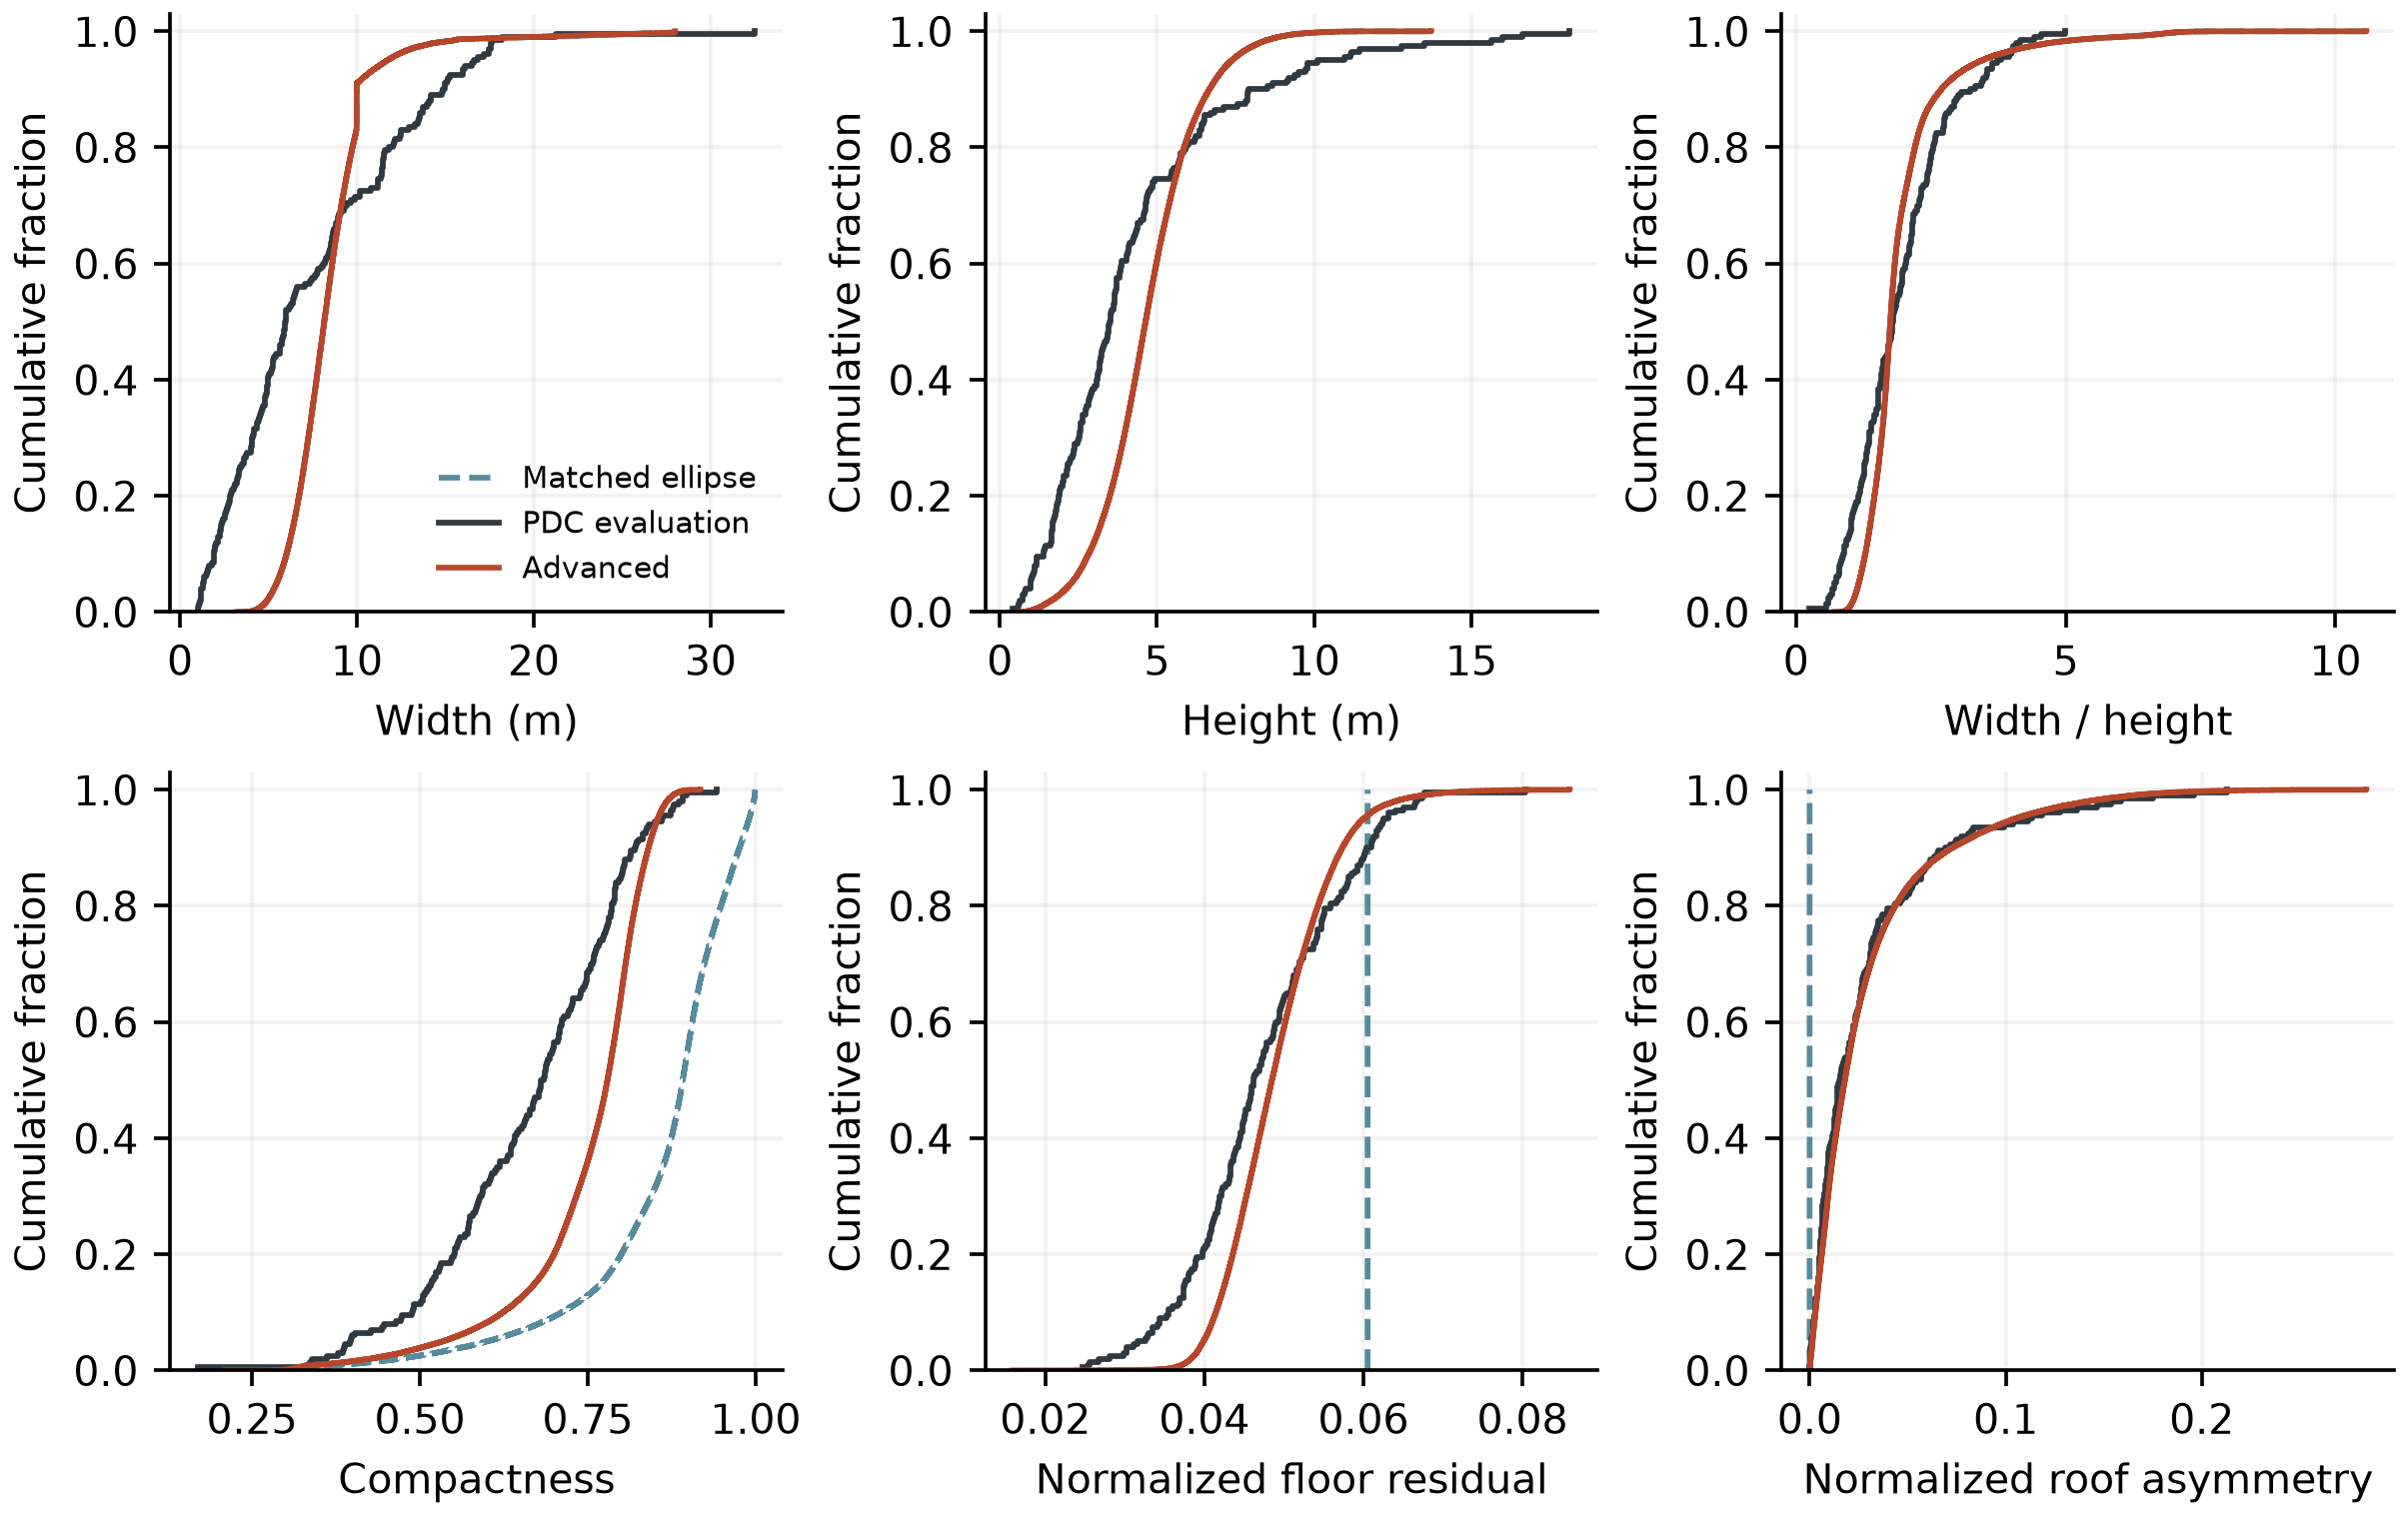
\includegraphics[width=0.96\textwidth]{figures/f09_morphometry.png}
\caption{Measured section-weighted descriptor distributions for 200 PDC evaluation contours from 19 caves and 118,257 generated profiles from 100 Earth worlds. Advanced and matched-ellipse curves coincide for width, height and aspect ratio by construction. The closer floor-residual and roof-asymmetry distributions accompany remaining size and compactness mismatches. These are input-profile comparisons; they do not validate the reconstructed mesh.}
\label{fig:morph-evaluation}
\end{figure*}

\subsection{Controllability, Ablation, and Sampling}
All 700 routing cases completed, giving 100 valid seed pairs per intervention (Table~\ref{tab:ablation}). Single-term removals produced median symmetric centerline displacements of 4.79--8.34 m; constant routing cost produced 12.39 m. These distances measure a changed route, not improved geological agreement.

Cycle-rank responses were less uniform. Paired median changes were zero for cover, capacity and stability removal, $+1$ for slope removal, and $-1$ for fracture removal. Their intervals included zero. Constant routing cost increased cycle rank by a median 1.5, with interval [1, 2]. The full model's median cycle rank was 12. Differences between condition medians are not substituted for paired effects: for example, capacity removal has condition median 11.5 but paired median change zero.

All 1,200 control cases completed, giving 100 valid high-versus-low seed pairs for each control. Raising duration from 0.5 to 1.5 increased main-route length by a paired median 3.810 km, with 95\% interval [3.682, 4.929] km. Raising inflation from 0.2 to 0.8 increased the junction-to-passage width ratio by 0.0318 [0.0162, 0.0490], a modest response. Distributary tendency from 0.2 to 0.8 produced a paired median cycle-rank change of zero [0, 0]; all three level medians were 12. This does not support an increase in the declared primary topology readout and does not establish that individual graphs were unchanged. Supply from 0.7 to 1.3 changed resolved host scale from 0.837 to 1.140 in every seed. That deterministic input-resolution response is not independent evidence of generated geometric control. These results support only partial control of the declared readouts.

All 30 sampling cases completed. Adaptive sampling had a larger pooled mean boundary-point discrepancy in every pair: median 2.296 m, versus 1.861 m for uniform sampling. The median paired increase was 0.439 m, with 95\% interval [0.432, 0.454] m. The paired increase in 95th-percentile discrepancy was 2.107 m [2.066, 2.169]. Counts were approximate rather than exact matches: median adaptive count was 1,198.5, versus 1,227 for uniform and 9,911.5 for the reference. The paired count change was $-29.5$ [$-32$, $-27$]. This experiment does not support a sampling advantage under its point-set metric. The unequal counts and density-sensitive metric also prevent interpreting the result as a continuous-surface or final-mesh accuracy comparison.

\begin{table}[t]
\caption{Paired routing-term effects relative to the full model. Values are median paired changes; brackets give pointwise 95\% bootstrap intervals. Each intervention has 100 valid pairs.}
\label{tab:ablation}
\centering\small
% Source summary SHA256: f9a174b94102267422a2b95ff694b8341572fc496f97bd76ad7da059695ae683
\begin{tabularx}{\columnwidth}{@{}Yccc@{}}
\toprule
Condition & Pairs & Shift (m) & $\Delta\beta_1$ \\
\midrule
No slope term & 100 & \shortstack[r]{$8$\\\scriptsize $[7.19, 8.86]$} & \shortstack[r]{$1$\\\scriptsize $[0, 2]$} \\
No cover term & 100 & \shortstack[r]{$4.79$\\\scriptsize $[4.04, 5.44]$} & \shortstack[r]{$0$\\\scriptsize $[0, 0]$} \\
No fracture term & 100 & \shortstack[r]{$8.34$\\\scriptsize $[7.57, 9.59]$} & \shortstack[r]{$-1$\\\scriptsize $[-1, 0]$} \\
No capacity term & 100 & \shortstack[r]{$6.93$\\\scriptsize $[5.87, 8.27]$} & \shortstack[r]{$0$\\\scriptsize $[-1, 0]$} \\
No stability term & 100 & \shortstack[r]{$5.71$\\\scriptsize $[5, 6.55]$} & \shortstack[r]{$0$\\\scriptsize $[-1, 0]$} \\
Constant cost & 100 & \shortstack[r]{$12.4$\\\scriptsize $[11.4, 13]$} & \shortstack[r]{$1.5$\\\scriptsize $[1, 2]$} \\
\bottomrule
\end{tabularx}

\end{table}

\subsection{Resource Use and Export Evidence}
All 40 resource cases were attempted: 35 completed and five reached the monitored memory limit (Table~\ref{tab:scale} and Figure~\ref{fig:resource-evaluation}). Tiled storage completed all 20 cases, including the five requested 5 km routes, with median time 126.7 s and peak RSS 1.65 GiB at that size. Dense storage completed all cases through 2 km but exceeded the 12 GiB budget in every 5 km case. Its median peak RSS at 2 km was 10.90 GiB, compared with 1.03 GiB for tiled storage. Tiling did not consistently reduce time: the two modes had similar medians at 2 km, while tiled medians were higher at 0.5 and 1 km. Stopped dense runs are not assigned a completion time or used to calculate a 5 km speedup.

These measurements include network construction through finalized meshing at 0.6 m voxel spacing, excluding optional events, rocks, appearance and export. Requested route length is a configuration target. Realized dominant routes ranged from 0.521--0.661 km for the 0.5 km request to 5.174--5.487 km for the 5 km request; branches add further length. The five 5 km tiled meshes contained 1.31--1.53 million faces. Completion is not a fidelity criterion: among 17,634 input profiles from the 20 distinct benchmark worlds, 10,248 (58.1\%) had fewer than eight voxels across their smallest dimension. Completed meshes had one, three or four surface components; void grids had one, two, four or five components. These counts identify cases for continuity inspection, without establishing the cause or whether each component is unintended. No local mesh-cut or resolution-convergence study was executed, and the benchmark roof screen inserted no collapse plugs.

\begin{table}[t]
\caption{Measured reconstruction costs at 0.6 m voxel spacing. Time and memory are medians over completed cases; denominators include all attempts. All five 5 km dense runs exceeded the 12 GiB memory budget, so their completion costs are unavailable.}
\label{tab:scale}
\centering\small
% Source summary SHA256: e5a493bc3896c4f9881cdcd892e89eabcd6e7eb1cd6bb7bd7c7b9d82b291b7dc
\begin{tabularx}{\columnwidth}{@{}Ylccc@{}}
\toprule
Route (km) & Mode & Complete & Time (s) & RSS (GiB) \\
\midrule
0.5 & Dense & 5/5 & 29.2 & 1.72 \\
0.5 & Tiled & 5/5 & 34.9 & 0.497 \\
1 & Dense & 5/5 & 49 & 3.98 \\
1 & Tiled & 5/5 & 51.5 & 0.735 \\
2 & Dense & 5/5 & 73.3 & 10.9 \\
2 & Tiled & 5/5 & 73.7 & 1.03 \\
5 & Dense & 0/5 & \textemdash & \textemdash \\
5 & Tiled & 5/5 & 127 & 1.65 \\
\bottomrule
\end{tabularx}

\end{table}

\begin{figure*}[t]
\centering
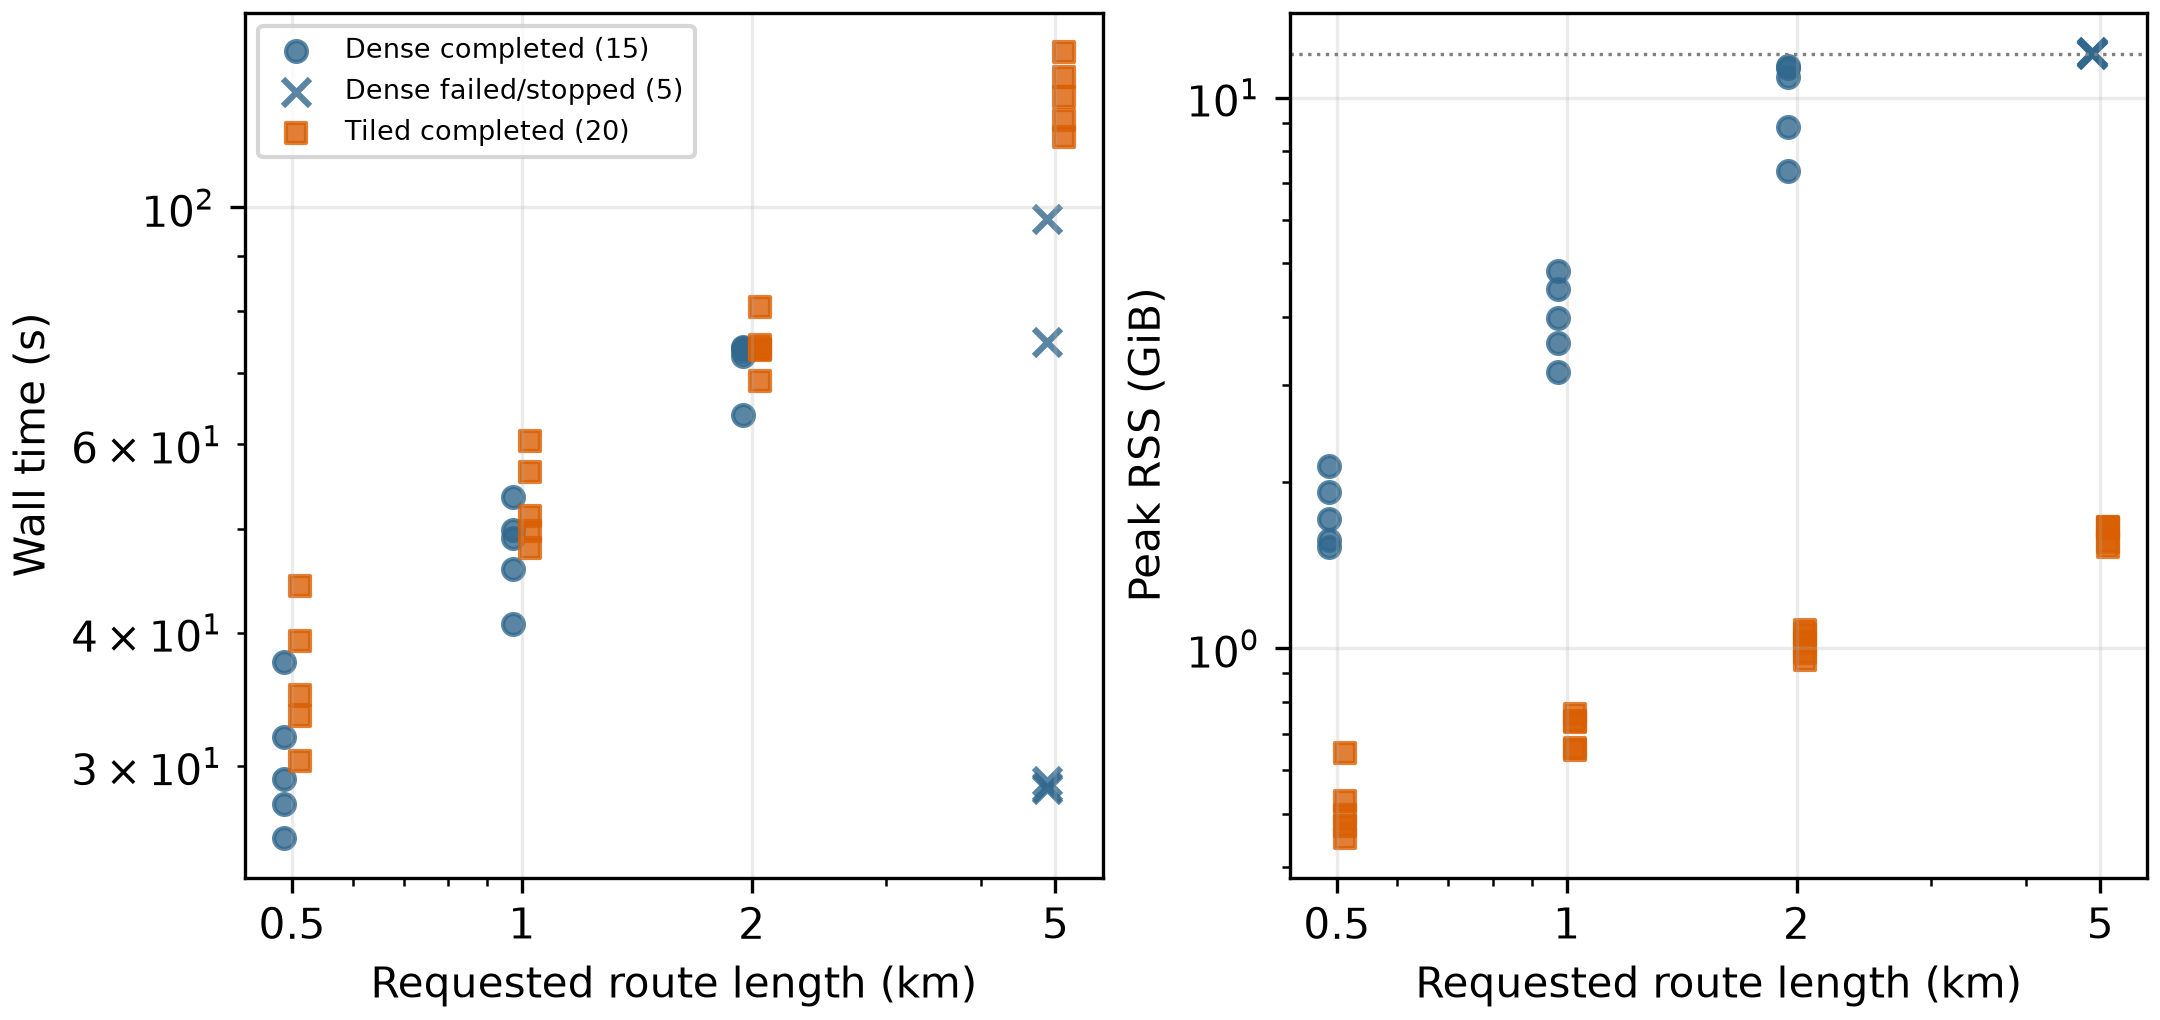
\includegraphics[width=0.96\textwidth]{figures/f10_scalability.png}
\caption{All 40 resource measurements on the campaign workstation, with five seeds per size and storage mode. Circles and squares show completed dense and tiled reconstructions; crosses show resource use when dense runs were stopped, not completion costs. The dotted line marks the monitored 12 GiB budget. Axes are logarithmic, with a small horizontal offset separating storage modes at each requested length. Scope is host generation through finalized meshing at 0.6 m, excluding optional events, props, appearance and exports.}
\label{fig:resource-evaluation}
\end{figure*}

All three export worlds completed, emitting 15 target packages with visual and collision assets present. Their configuration identities were verified against the original frozen package. The automatic bounds parser inspected nine GLB assets across Blender, UE5 and Unity; the maximum relative extent discrepancy was $1.74\times10^{-3}$ (0.174\%). Gazebo package and Omniverse USD bounds were not parsed. These comparisons include the shared visual-surface preparation described above and cannot isolate transform accuracy. No application imports, material inspections or dynamic contact tests were completed; package presence is the scope of the recorded export pass flag.

All 11 A--C repeatability and stage-isolation checks passed for each of three seeds, giving 33 successful checks. Host, network and section semantic hashes matched repeated generation and the declared downstream-setting interventions; the section checkpoint was reused and preserved its semantic hash. This evidence is limited to the recorded environment and A--C artifacts. Final meshes, exported container bytes and cross-platform repeatability were not tested by this suite.

\subsection{Failure Analysis}
The only recorded execution failures were the five dense 5 km reconstructions that reached the memory budget: 5/40 resource attempts, and 5/2,076 campaign cases. No case timed out. All selected reference contours were retained, and the network/profile suites completed their declared cases. Completion nevertheless coexists with limitations: absolute profile dimensions remain mismatched, adaptive sampling has greater point-set discrepancy, the distributary readout has no median response, and coarse reconstructions contain under-resolved profiles and multiple components. Unperformed application imports are missing evidence, not successful or failed imports. The report keeps these distinct from execution exceptions.

\section{Discussion}
\subsection{What the Representation Makes Testable}
PLUME-Advanced exposes relationships that are difficult to examine in a mesh-only workflow. Routing terms can be varied and measured; graph alternatives can be compared with final geometric connectivity; profile sampling can be studied without changing the intended network; and exported assets can be traced to a canonical source. The measured routing shifts, partial control responses and negative sampling result demonstrate why these representations need separate readouts. Their usefulness for an autonomy system remains a question for robotics experiments.

Separating formation, survival, and traversability also makes negative results interpretable. A route may be proposed because the host favors it and then blocked because its actual span and cover fail the local screen. A surviving passage may still violate a robot's clearance. Treating all three outcomes as one ``valid cave'' flag would obscure the responsible mechanism. The retained artifacts instead support attributing a rejection to a particular modelling or representation stage.

\subsection{Empirical Validity and Calibration}
Terrestrial descriptor agreement is one component of plausibility. Marginal distributions can agree even when their joint relationships are wrong: for example, matching width and height separately does not ensure the correct relationship between aspect ratio, floor form, and chamber size. Cross-sectional agreement also says little about longitudinal persistence, spatial covariance, entrance frequency, or network topology. Additional validation could examine joint descriptors, survey-level trends, and independent three-dimensional scans.

The current matched ellipse is intentionally simple and isolates nonelliptical profile structure. It cannot establish superiority over other complete generators. Direct comparison with empirically parameterized software would require controlling the task and separating parameter fitting from evaluation. Statistical profile families learned from reference sections could later replace individual procedural shape controls while preserving the host, network, and export architecture.

Calibration and scenario design also have different purposes. A morphology prior fitted to observed terrestrial sections can support an Earth comparison, whereas a deliberately difficult robotics benchmark may emphasize rare junctions, narrow clearances, or alternative routes. The latter is useful when declared, but its distribution should not be described as the natural frequency of lava-tube features. The same caution applies to event preservation rules and selection of visually attractive seeds.

\subsection{Planetary Extrapolation and Model Limits}
The Moon and Mars presets combine gravity, material assumptions, passage envelopes, host correlation scales, and network controls. Their outputs are scenario extrapolations, not reconstructions of measured interiors. A same-seed body comparison illustrates changes under an entire preset. Isolating gravity requires a different experiment in which material, formation dimensions, and other controls are held fixed.

The host is a spatial prior, flow state is procedural bookkeeping, and the beam screen is a restricted local constraint. Static events do not simulate fracture propagation, dynamic collapse, sediment transport, or granular contact. The two-dimensional host cannot capture arbitrary buried stratigraphy. Surface materials are not a calibrated sensor model. These limits restrict geological and robotics conclusions independently: plausible cave shape does not establish a realistic radar return, and accurate package scale does not establish realistic wheel--terrain interaction.

\subsection{Use in Robotics Experiments}
The framework supplies environments rather than an autonomy system. A useful robotics evaluation would freeze a robot model, sensors, start and goal selection, and compute budget, then compare algorithms across held-out environment seeds. Training, tuning, and test environments should be partitioned at the world level. Reusing sections or subregions from the same world across partitions can leak distinctive geometry and inflate apparent generalization.

Relevant outcomes include localization error, exploration coverage, path cost, collision frequency, recovery behavior, and communication-related mission completion. These should be measured from simulated missions, not inferred from graph statistics. An increased cycle rank creates route alternatives, but whether it helps an exploration policy depends on sensing, loop closure, traversability, and resource constraints.

For planners and traversability estimators, the intrinsic atlas offers segment-indexed floor samples and a link back to world geometry. It is privileged scene information. Experiments must state whether an algorithm receives this information as an oracle, uses it only for evaluation, or reconstructs an estimate from sensors. Providing the generator's full topology to one method while withholding it from another changes the task and can confound comparisons.

\subsection{Reproducibility and Release Scope}
The dated campaign record retains source snapshots, project inputs, seed lists, cave partitions, dependency versions, case records and their hashes, descriptor tables, summaries, execution logs and figure-generation inputs. Per-case configuration and provenance identities were reconstructed and checked against all 2,076 records. All 136 original snapshot files, 137 amended snapshot files and four referenced texture files matched their recorded hashes at the end. The exporter produced 111 files, whose content hashes are also recorded. Source data and texture assets remain separately identified external inputs.

The compact manuscript package includes the measurement tables and source records needed to audit the reported numbers. Large contour arrays and emitted scene packages remain in the repository's campaign outputs; benchmark meshes were measured in their worker processes rather than retained as a mesh archive. Earlier figures retain their schematic or development status, while Figures~\ref{fig:morph-evaluation} and~\ref{fig:resource-evaluation} use campaign data. There was no generator fitting to these outcomes. Future calibration or algorithm changes require a new versioned study; they do not replace the negative results of this one.

\section{Conclusion}
PLUME-Advanced provides a staged procedural framework for constructing lava-tube environments with explicit host conditioning, directed network semantics, adaptive three-dimensional sections, volumetric structural changes, and portable scene packaging. A refreshed intrinsic floor atlas preserves segment identity and vertical level while exposing the consequences of changes to the cave volume. The architecture distinguishes a proposed formation network from the surviving void and from robot-specific traversability.

The Earth campaign found closer selected shape descriptors than matched ellipses and lower memory use with tiled reconstruction, alongside persistent size mismatch and unresolved mesh-fidelity questions. Parameter responses were partial, and the sampled-point comparison did not support an adaptive-sampling advantage. Repeatability and package checks passed within their stated scope. These findings support an inspectable environment prior for controlled studies rather than validated planetary interiors or demonstrated robotics benefits. Future work includes calibration on the designated calibration data, stronger control semantics, continuous-surface and final-mesh validation, actual simulator imports, geology-conditioned appearance, explicit entrances and skylights, and evaluation of robotic autonomy across declared scenarios.

\FloatBarrier
\appendices
\section{Supplementary Scenario Comparison}
\label{app:bodies}
The gravity comparison in Figure~\ref{fig:roof-screen} isolates one structural input while holding material properties fixed. A future full Earth, Mars, and Moon preset comparison should additionally identify the changed formation and representation parameters, use matching seeds and visualization conventions, and show each panel's metric scale. It is not included as a measured result in this draft.



\section{Minimum Evidence Attached to a Final Figure}
Every measured figure should identify its experiment, source files, model/configuration revision, seed or seed set, coordinate system, units, and status of excluded or failed cases. Distribution plots need sample counts at both the section and cave/world levels. Paired interventions need valid-pair counts. Error bars need an estimand and resampling unit. Geometry comparisons need the same location and a shared scale; application screenshots need version and import evidence.

Method diagrams can be authored directly from the architecture and labelled as schematics. Existing diagnostic renders can supply illustration panels, but their labels and captions must describe what is actually visible. A rock-placement image is not a before/after collapse experiment, and a plan-view floor map without overlapping levels is not evidence that a multilevel crossing has been resolved. Measured results must never be replaced by plausible-looking synthetic charts.

\begin{thebibliography}{99}

\bibitem{sauro2020}
F. Sauro, R. Pozzobon, M. Massironi, P. De Berardinis, T. Santagata, and J. De Waele,
``Lava tubes on Earth, Moon and Mars: A review on their size and morphology revealed by comparative planetology,''
\emph{Earth-Science Reviews}, vol. 209, Art. no. 103288, 2020,
doi: \href{https://doi.org/10.1016/j.earscirev.2020.103288}{10.1016/j.earscirev.2020.103288}.

\bibitem{carrer2024}
L. Carrer, R. Pozzobon, F. Sauro, D. Castelletti, G. W. Patterson, and L. Bruzzone,
``Radar evidence of an accessible cave conduit on the Moon below the Mare Tranquillitatis pit,''
\emph{Nature Astronomy}, 2024,
doi: \href{https://doi.org/10.1038/s41550-024-02302-y}{10.1038/s41550-024-02302-y}.

\bibitem{cano_navigation}
L. Cano, A. R. Mosteo, and D. Tardioli,
``Navigating underground environments using simple topological representations,''
in \emph{Proc. IEEE/RSJ International Conference on Intelligent Robots and Systems (IROS)},
2022, pp. 1717--1724,
doi: \href{https://doi.org/10.1109/IROS47612.2022.9981336}{10.1109/IROS47612.2022.9981336}.

\bibitem{daedalus2021}
A. P. Rossi, F. Maurelli, V. Unnithan, \emph{et al.},
``DAEDALUS---Descent And Exploration in Deep Autonomy of Lava Underground Structures,''
W\"urzburger Forschungsberichte in Robotik und Telematik, no. 21,
Universit\"at W\"urzburg, 2021.

\bibitem{plume2025}
G. M. Garcia, A. Richard, and M. A. Olivares-Mendez,
``PLUME: Procedural Layer Underground Modeling Engine,''
in \emph{Proc. International Conference on Space Robotics (iSpaRo)}, 2025.
Available preprint: \href{https://arxiv.org/abs/2508.20926}{arXiv:2508.20926}.
% The supplied conference attribution is retained. Before submission, reconcile
% the final publisher pagination/DOI with the author's publication record.

\bibitem{blair2017}
D. M. Blair, L. Chappaz, R. Sood, C. Milbury, H. J. Melosh, K. C. Howell, and A. M. Freed,
``The structural stability of lunar lava tubes,''
\emph{Icarus}, vol. 282, pp. 47--55, 2017,
doi: \href{https://doi.org/10.1016/j.icarus.2016.10.008}{10.1016/j.icarus.2016.10.008}.

\bibitem{chwala2024}
M. Chwa\l{}a, G. Komatsu, and J. Haruyama,
``Structural stability of lunar lava tubes with consideration of variable cross-section geometry,''
\emph{Icarus}, vol. 411, Art. no. 115928, 2024,
doi: \href{https://doi.org/10.1016/j.icarus.2023.115928}{10.1016/j.icarus.2023.115928}.

\bibitem{johnson2010}
L. Johnson, G. N. Yannakakis, and J. Togelius,
``Cellular automata for real-time generation of infinite cave levels,''
in \emph{Proc. Workshop on Procedural Content Generation in Games}, 2010,
doi: \href{https://doi.org/10.1145/1814256.1814266}{10.1145/1814256.1814266}.

\bibitem{santamaria2014}
A. Santamar\'ia-Ibirika, X. Cantero, M. Salazar, J. Devesa, I. Santos, S. Huerta, and P. G. Bringas,
``Procedural approach to volumetric terrain generation,''
\emph{The Visual Computer}, vol. 30, pp. 997--1007, 2014,
doi: \href{https://doi.org/10.1007/s00371-013-0909-y}{10.1007/s00371-013-0909-y}.

\bibitem{antoniuk2016}
I. Antoniuk and P. Rokita,
``Procedural generation of underground systems with terrain features using schematic maps and L-systems,''
\emph{Challenges of Modern Technology}, vol. 7, no. 3, pp. 8--15, 2016.

\bibitem{paris2021}
A. Paris, E. Gu\'erin, A. Peytavie, P. Collon, and E. Galin,
``Synthesizing geologically coherent cave networks,''
\emph{Computer Graphics Forum}, vol. 40, no. 7, pp. 277--287, 2021,
doi: \href{https://doi.org/10.1111/cgf.14420}{10.1111/cgf.14420}.

\bibitem{cano_gazebo}
L. Cano, D. Tardioli, and A. R. Mosteo,
``Procedural generation of underground environments for Gazebo,''
in \emph{ROBOT2022: Fifth Iberian Robotics Conference},
Lecture Notes in Networks and Systems, vol. 590, 2023, pp. 314--324,
doi: \href{https://doi.org/10.1007/978-3-031-21062-4_26}{10.1007/978-3-031-21062-4\_26}.

\bibitem{pyroduct2026}
F. A. P. Romio, G. Lobosco, F. Sauro, R. Pozzobon, and A. Marraffa,
``Pyroduct: A novel parametric software for the simulation of terrestrial, lunar, and Martian lava tubes,''
\emph{Icarus}, vol. 447, Art. no. 116904, 2026,
doi: \href{https://doi.org/10.1016/j.icarus.2025.116904}{10.1016/j.icarus.2025.116904}.

\bibitem{pdc2025}
F. A. P. Romio, G. Lobosco, A. Marraffa, L. Pisani, and I. Tomasi,
``Pyroduct Digital Catalog,'' version 2.0, Zenodo, Nov. 2025.
Version-specific doi: \href{https://doi.org/10.5281/zenodo.17750755}{10.5281/zenodo.17750755};
recommended catalog citation: \href{https://doi.org/10.5281/zenodo.14535885}{10.5281/zenodo.14535885}.

\bibitem{marching1987}
W. E. Lorensen and H. E. Cline,
``Marching cubes: A high resolution 3D surface construction algorithm,''
in \emph{Proc. SIGGRAPH}, 1987, pp. 163--169,
doi: \href{https://doi.org/10.1145/37401.37422}{10.1145/37401.37422}.

\end{thebibliography}

\end{document}
